\documentclass[12pt,a4paper]{article} %,twocolumn
\usepackage[utf8]{inputenc}
\usepackage{amsmath}
\usepackage{amsfonts}
\usepackage{amssymb}
\usepackage{graphicx}
\usepackage{hyperref}
\usepackage{multicol, caption}
\usepackage{wrapfig}
\newenvironment{Figure}
  {\par\medskip\noindent\minipage{\linewidth}}
  {\endminipage\par\medskip}
\usepackage{listings}
\usepackage{color}
\definecolor{mygreen}{rgb}{0,0.6,0}
\definecolor{mygray}{rgb}{0.5,0.5,0.5}
\definecolor{mymauve}{rgb}{0.58,0,0.82}
\usepackage[table,xcdraw]{xcolor}
\lstset{ 
  backgroundcolor=\color{white},   % choose the background color; you must add \usepackage{color} or \usepackage{xcolor}; should come as last argument
  basicstyle=\footnotesize,        % the size of the fonts that are used for the code
  breakatwhitespace=false,         % sets if automatic breaks should only happen at whitespace
  breaklines=true,                 % sets automatic line breaking
  captionpos=b,                    % sets the caption-position to bottom
  commentstyle=\color{mygreen},    % comment style
  deletekeywords={...},            % if you want to delete keywords from the given language
  escapeinside={\%*}{*)},          % if you want to add LaTeX within your code
  extendedchars=true,              % lets you use non-ASCII characters; for 8-bits encodings only, does not work with UTF-8
  frame=single,	                   % adds a frame around the code
  keepspaces=true,                 % keeps spaces in text, useful for keeping indentation of code (possibly needs columns=flexible)
  keywordstyle=\color{blue},       % keyword style
  language=Python,                 % the language of the code
  morekeywords={*,...},            % if you want to add more keywords to the set
  numbers=left,                    % where to put the line-numbers; possible values are (none, left, right)
  numbersep=5pt,                   % how far the line-numbers are from the code
  numberstyle=\tiny\color{mygray}, % the style that is used for the line-numbers
  rulecolor=\color{black},         % if not set, the frame-color may be changed on line-breaks within not-black text (e.g. comments (green here))
  showspaces=false,                % show spaces everywhere adding particular underscores; it overrides 'showstringspaces'
  showstringspaces=false,          % underline spaces within strings only
  showtabs=false,                  % show tabs within strings adding particular underscores
  stepnumber=1,                    % the step between two line-numbers. If it's 1, each line will be numbered
  stringstyle=\color{mymauve},     % string literal style
  tabsize=2,	                       % sets default tabsize to 2 spaces
  title=\lstname                   % show the filename of files included with \lstinputlisting; also try caption instead of title
}
\usepackage{pgf,tikz,pgfplots}
\pgfplotsset{compat=1.15}
\usepackage{mathrsfs}
\usetikzlibrary{arrows}
\usepackage[left=2cm,right=2cm,top=3cm,bottom=3cm]{geometry}
%\usepackage{biblatex} %Imports biblatex package

\usepackage{fancyhdr}
 
\pagestyle{fancy}
\fancyhf{}
\rhead{Bachelorproject 2019}
\lhead{Analyzing protein sequences with Deep Neural Networks}
\cfoot{\thepage}

\author{Rasmus Porse Bjørneskov\\Roald Frej Vitus Simonsen}
\title{Analyzing protein sequences with Deep Neural Networks} 
\begin{document}
\definecolor{qqttcc}{rgb}{0,0.2,0.8}
\definecolor{qqffqq}{rgb}{0,1,0}
\definecolor{ffqqqq}{rgb}{1,0,0}
\maketitle
\section*{Abstract}
In this paper we explore the theory underlying proteins and features of the amino acids they are comprised of, exploring aspects such as secondary protein structures and solvent accessibility.\\
We then delve into the theory behind artificial neural networks, deliberating basic subjects such as the structure of neural networks and \textit{backprobagation}, as well as explaining the extentions to this concept called \textit{convolutional neural networks} and \textit{multi-task learning}.\\
We then introduce a dataset originally produced by 
\newpage
\tableofcontents
\newpage
\begin{multicols}{2}
\section{Introduction}
Before presenting the motivation for this paper and the concepts used throughout it, we would like to elaborate on the purpose of the thesis. In our initial contract we have the following description of the purpose of the paper in Danish:\\\\
\textit{The purpose of this project is to learn how neural networks are based theoretically, to learn how they can be applied to solve specific tasks (in this case to predict protein properties based on their composition of amino acids) as well as achieving a basic understanding of these features. \\\\
We expect the process to have the following parts:\\
- Implementing a rudimentary neural network without use of newer tools, with the motivation to be able to explain the theoretical background for it.\\
- A real implementation of a artificial neural network based on established frameworks, such as PyTorch, with the motivation to be able to predict protein secondary structures, based on sequences of amino acids. \\
- A similar implementation with the motivation of being able to predict Solvent Accessible Surface Area based on amino acid sequences. \\
- A comparison of result from the two above mentioned models, contrasted with a model that uses multi-task learning to predict both of those properties.\\ }\\
Using this description as a guide through our work, we started with a look at a rudementary implentation of a neural network. As a starting point for this, we were given a Jupyter-notebook with some introductory explanations and excercises to do developed by Denny \citeauthor{britz}.\\
After completing the excercises and tweaking the code to get a better understanding of the methods and concepts, we afterwards implemented the same neural network using the library PyTorch on top of Python. 
This gave us a basic understanding of where to start coding our real neural networks. As it was used as a practice exercise for us to get started and achieve a basic level of understanding, we have not included the code or excersises in the paper.

\subsection{Motivation}
In computer science today, one of the areas of research that is publicly debated and covered by media and politicians alike, is the subject of Artificial Intelligence. Within this matter concepts like deep learning, machine learning and neural networks are showing up repeatedly as both publicly used buzzwords and central areas for future research and use.\\
This paper's purpose is threefold. The first is to give an introductory understanding of the topic of machine learning and more specifically neural networks. This includes a basic understanding of the theoretical basis of neural networks. \\
The second purpose is to widen this understanding of neural networks by implementing one to handle a specific task. This task is to predict secondary structure of proteins based on their amino acid composition. Lastly the purpose is to give a rudimentary understanding of what proteins and their composites are, to give context to the use of the neural network.\\
The motivation for choosing protein secondary structure prediction for the neural networks also has several reasons. \\
Protein secondary structure prediction has many real world applications and is an important branch of bioinformatics today, as it is used in both medicine, biotechnology and research into diseases such as Alzheimer's. \\
Improving predictive capabilities in regards to protein secondary structure is, at the time of writing, a very active area of research. As such it gives a contemporary and relevant context for this paper as an interesting introduction to neural networks and their application.   
A common example when learning about neural networks and implementing them is to identify a handwritten number between 0 and 9. This neural network is often trained on the MNIST dataset of handwritten numbers. \\
We will use the MNIST dataset of numbers to explain some of the basics of neural networks. 


\subsection{Proteins}
Proteins are large bio-molecules that serve a wide range of functions in organisms. Those functions includes giving structure to cells, being part of DNA replication and responding to stimuli. KILDEKILDEKILDE!!. They consist of chains of amino acids, the sequence of which determine the type of the protein. The linear sequence of amino acids in a protein is also known as a protein's primary structure. 

\subsubsection{Secondary Structures}
The secondary structures are the three-dimensional forms a protein can take in a local segment and are largely determined by its primary structure. There exists many reasons for research into predicting the secondary structure. One of these is using it as a stepping stone for trying to find the three-dimensional tertiary structure of a protein (which is normally difficult to assess). The secondary structure itself is the three-dimensional form of local segments of the protein \citep[p.~2]{qi-et-al-2012}.
The secondary structure is divided into groups of either 3 or 8 types of structure, named Q3 and Q8 \citep{zhou-and-troyanskaya-2014}. 
Using the DSSP alphabet \citep{kabsch-and-sander-1983} 
for giving the groups letters, the categories of Q8 are as shown in the Q8 table \citep{qi-et-al-2012}.
\begin{table}[H]
\caption{Q8 structure overview}
\centering
\begin{tabular}{l|l}
\hline 
Letter	& Secondary Structure 			\\ \hline
H	& Alpha-helix						\\
B	& residue in isolated beta bridge	\\
E	& extended strand					\\
G	& 3-helix							\\
I	& 5-helix							\\
T	& hydrogen bonded turn				\\
S	& bend								\\
L	& loop								\\
\end{tabular}
\end{table}
\noindent The accuracy for current state of the art when predicting Q8 secondary structure is around 72-76\% \citep{zhou-and-troyanskaya-2014, qi-et-al-2012, wang-et-al-2016}. \\
When predicting Q3 secondary structures the accuracy percentage of the current state of the art lies in the mid eighties. This was for a long time the main focus of research in secondary structure prediction, but due to recent advances in technology and research, the harder but more specific Q8 predictions are gaining more attention. 
Again using the DSSP alphabet for giving letters, the groups of Q3 are as in the Q3 table \citep{qi-et-al-2012}.
\begin{table}[H]
\caption{Q3 structure overview}
\centering
\begin{tabular}{l|l}
\hline
Letter		& Q8 structures in group	\\ \hline
H	(helix)		& H, G						\\
B	(sheet)		& B, E						\\
C (coil)	    & I, S, T, L				\\
\end{tabular}
\end{table}


\subsubsection{Solvent accessible surface area}
Another feature of proteins this paper shall examine, is amino acid solvent accessible surface area. This solvency is a measure of whether or not it can be absolved by water. Among other things this is determined by whether or not the acid is deep inside the protein or close to the surface of the protein. \\
This shall serve as the secondary task for the implementation of a multi-task learning model.

\subsection{Neural networks}
The common perception is that humans and animals process information, i.e. transform perceptional 
stimuli and physiological conditions into behaviour, by using their brains. This is imprecise 
however, as the brain as such is only one functioning part of what is called the \textit{nervous 
system}, which is in turn responsible for the internal workings of human and animal behaviour.\\
This nervous system is an abstaction over a number of \textit{neurons} interconnected by 
synapses. Neurons in turn are so-called electrically exitable cells. In a gross over-simplification, this can be explained as such: each neuron can have different internal states, depending on the internal states of the neurons it is connected to, thus forming a \textit{neural network}.

%\begin{figure}[h]
%  \centering
%  \frame{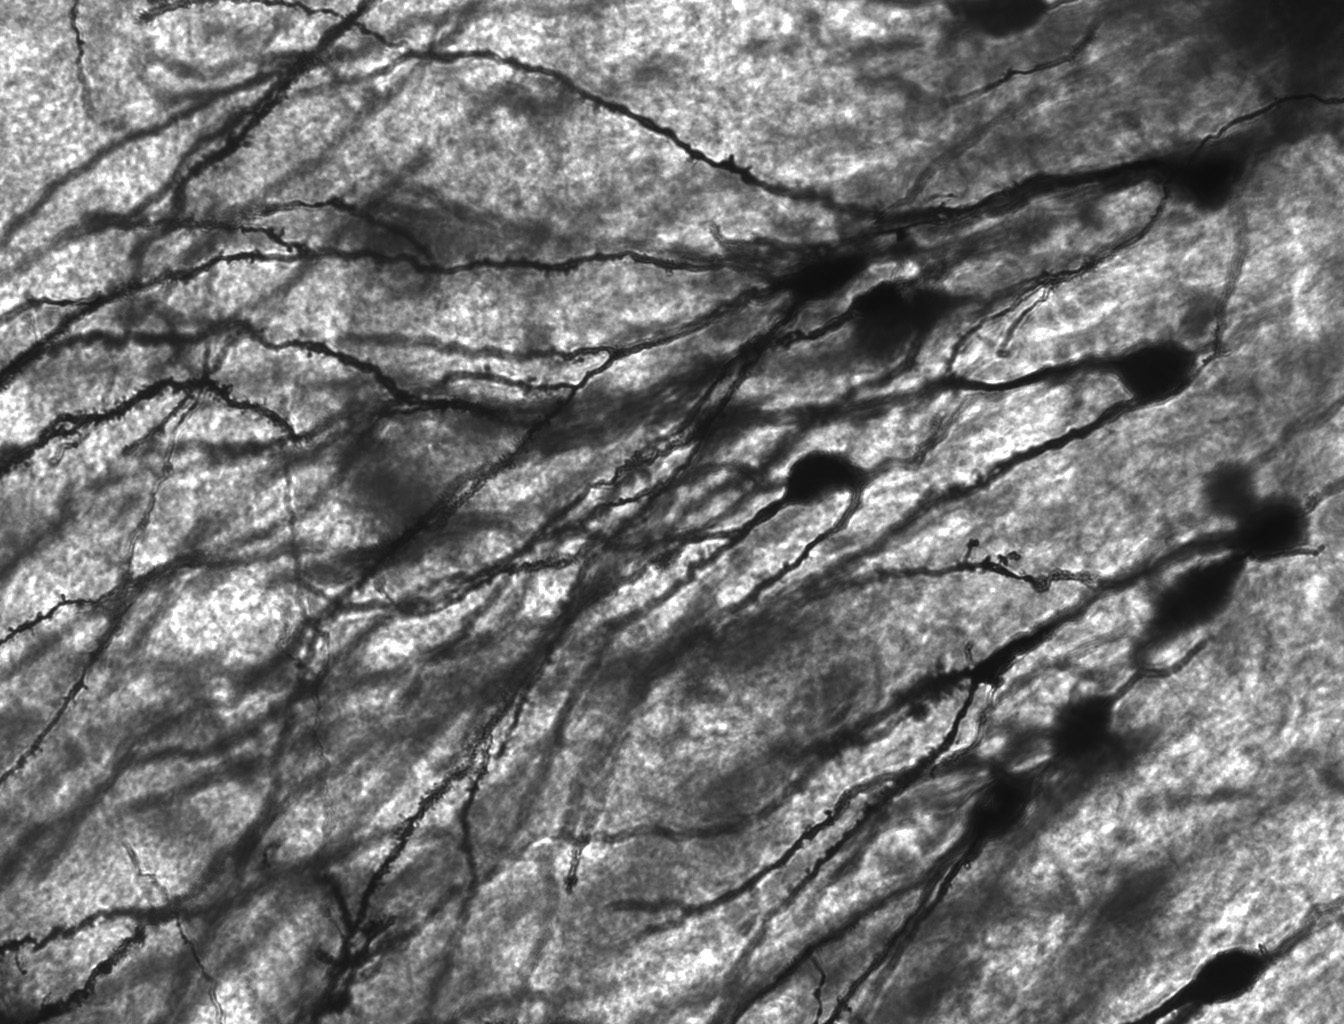
\includegraphics[width=0.8\linewidth]{images/Gyrus_Dentatus_40x}}
%  \caption{Neurons in the dentate gyrus of an epilepsy patient.}
%\end{figure}

\begin{Figure}
 \centering
 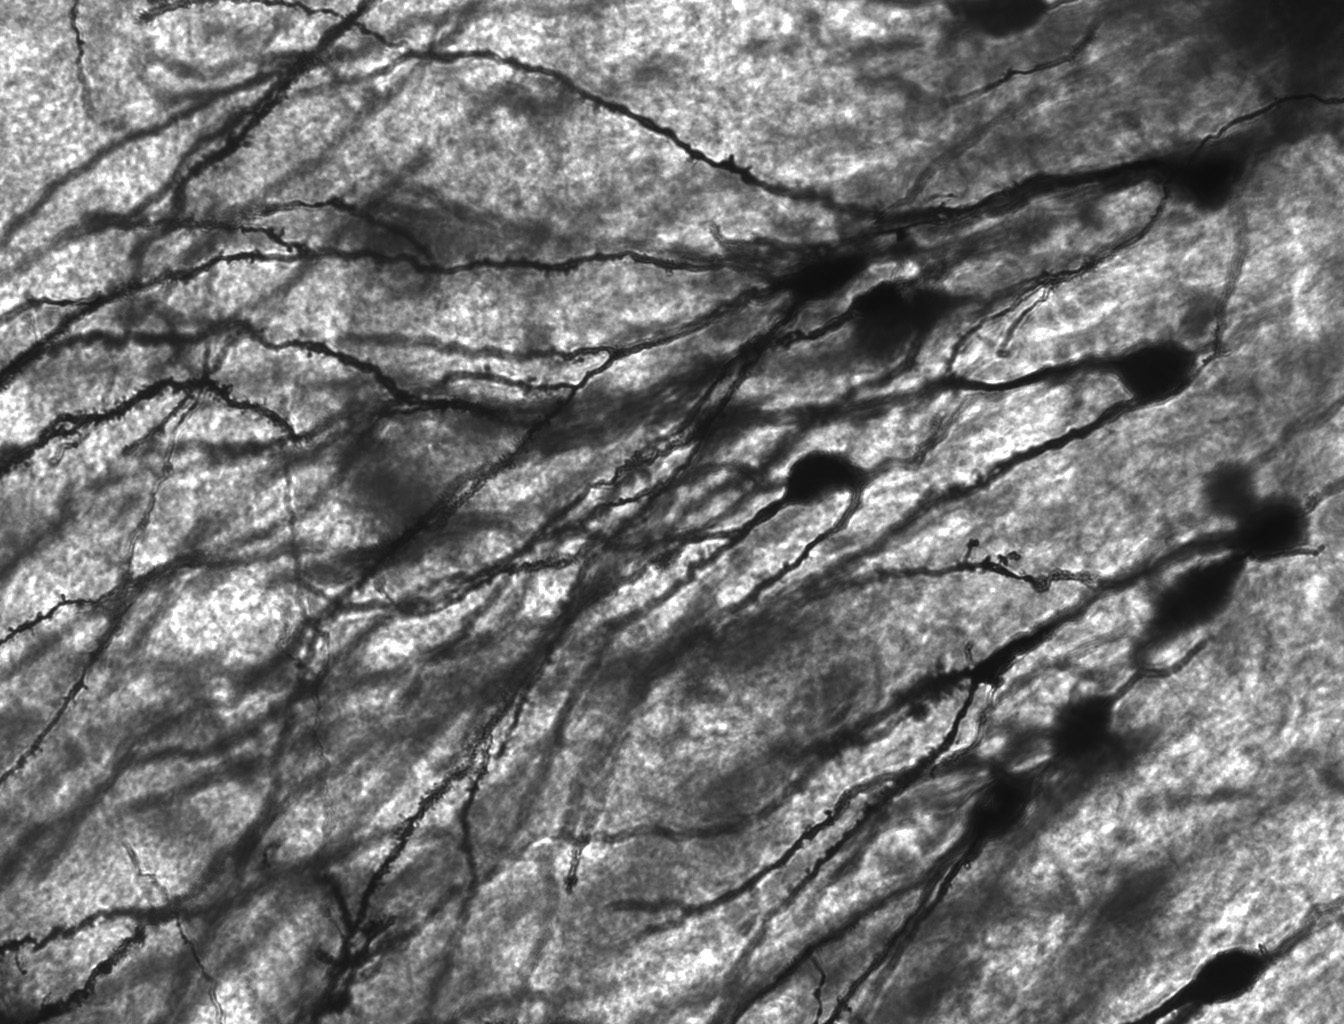
\includegraphics[width=0.8\linewidth]{images/Gyrus_Dentatus_40x}
 \captionsetup{width=0.8\linewidth, font=small}
 \captionof{figure}{Neurons in the dentate gyrus of an epilepsy patient.}
\end{Figure}

\noindent While obviously interesting within the fields of biology or psychology, this structure has shown 
to be useful in the field of computation, as one can in fact model this very 
thing and use it to make predictions based on prior observations, for example in regards to the 
aforementioned structures of proteins folding.\\
Analogously, or rather digienourmouslytally, we can use this model to construct an \textit{artificial 
neural network}.
These set themselves apart from biological neural networks in a couple of ways: neurons in biological neural networks are connected to each other via synapses. Each neuron has an either inhibitory or activating effect on whether or not a connected neuron 'fires'.\\
In contrast to this, artificial neural networks' neurons are connected by \textit{edges}, each with an associated \textit{weight}, allowing the artificial networks to leave the discrete domain and enter the continuous.

\subsubsection{Basics}
An artificial neural network is a specific instantiation of a \textit{multi-layer perceptron}.
A multi-layer perceptron in turn is a system of nodes arranged into layers and each receiving their value from the value of the nodes in the layer before them (adjusted by some weight) in combination with a bias (a scalar) and an activation function of some sort. \\
In this way the first layer will be called the \textit{input layer}, the last layer the \textit{output layer} and all layers in between \textit{hidden layers}. \\
In the case of neural networks, the nodes in the system are referred to as neurons.

\begin{Figure}
 \centering
 \begin{tikzpicture}[line cap=round,line join=round,>=triangle 45,x=0.4cm,y=0.4cm]
\clip(0,0) rectangle (15,15);
\draw [line width=1pt,fill=ffqqqq,fill opacity=1] (2,7) circle (0.4cm);
\draw [line width=1pt,fill=ffqqqq,fill opacity=1] (2,10) circle (0.4cm);
\draw [line width=1pt,fill=qqffqq,fill opacity=1] (7,4) circle (0.4cm);
\draw [line width=1pt,fill=qqffqq,fill opacity=1] (7,7) circle (0.4cm);
\draw [line width=1pt,fill=qqffqq,fill opacity=1] (7,10) circle (0.4cm);
\draw [line width=1pt,fill=qqffqq,fill opacity=1] (7,13) circle (0.4cm);
\draw [line width=1pt,fill=qqttcc,fill opacity=1] (12,10) circle (0.4cm);
\draw [line width=1pt,fill=qqttcc,fill opacity=1] (12,7) circle (0.4cm);
\draw [line width=1pt] (3,10)-- (6,13);
\draw [line width=1pt] (3,10)-- (6,10);
\draw [line width=1pt] (3,10)-- (6,7);
\draw [line width=1pt] (3,10)-- (6,4);
\draw [line width=1pt] (3,7)-- (6,13);
\draw [line width=1pt] (3,7)-- (6,10);
\draw [line width=1pt] (3,7)-- (6,7);
\draw [line width=1pt] (3,7)-- (6,4);
\draw [line width=1pt] (8,13)-- (11,10);
\draw [line width=1pt] (8,10)-- (11,10);
\draw [line width=1pt] (8,7)-- (11,10);
\draw [line width=1pt] (8,4)-- (11,10);
\draw [line width=1pt] (8,4)-- (11,7);
\draw [line width=1pt] (11,7)-- (8,7);
\draw [line width=1pt] (8,10)-- (11,7);
\draw [line width=1pt] (11,7)-- (8,13);
\end{tikzpicture}
 \captionsetup{width=0.8\linewidth, font=small}
 \captionof{figure}{An extremely simple neural network.}
\end{Figure}
\noindent The neural network shown consists of two input neurons (red), one hidden layer of three neurons (green) and two output neurons(blue). The black edges between the neurons represent the weights and biases of the system.\\
Thus, if one was to describe it more accurately, the value $z_i$ of neuron layer \textit{i} with \textit{d} number of neurons in it, given the matrix of sets of weights \textit{w} (the biases being the very first row) and the activation function $h()$ can be expressed as follows:
\[
z_i = h\left(\sum_{j=0}^d w_{ij}\cdot z_{i-1} + w_{i0}\right)
\]
Such a model is useful for calculating continuous values as well as for classification purposes. A common example of the latter is the MNIST data set of hand-written digits in 28x28 pixel greyscale images. In this case the light intensity of the 784 ($28^2$) pixels could fittingly be the input layer, while a layer consisting of 10 nodes (corresponding to digits 0 through 9) could be the output layer, such that the system could be used to predict which digit is written in a given image.
%\begin{figure}[h]
%  \centering
%  \frame{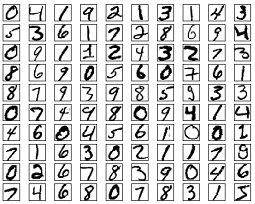
\includegraphics[width=0.7\linewidth]{images/mnist}}
%  \caption{Handwritten digits in the MNIST data set.}
%\end{figure}

\begin{Figure}
 \centering
 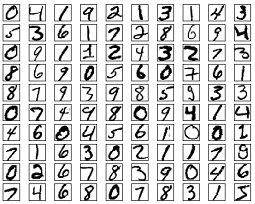
\includegraphics[width=0.7\linewidth]{images/mnist}
 \captionsetup{width=0.8\linewidth, font=small}
 \captionof{figure}{Handwritten digits in the MNIST data set.}
\end{Figure}

\noindent A common implementation of a neural network to perform this task is to have a single hidden layer of 800 nodes, however the most successful implementations in regards to the MNIST data set have been made with \textit{convolutional neural networks}, but we shall return to these later.

\subsubsection{Training}
Simply having defined the system of the neural network as above (denoted $f_{NN}$) naturally does not give a reliable method for classifying, as the accuracy of the prediction inherently depends on the correctness of the weights and biases of the system (denoted $\Theta$), which must be initialized with random values. \\
Enter a concept named \textit{backpropagation}. Having a set of predicted values ($\hat{y}$) for a data set (\textit{x}) along with the observed correct values (\textit{y}), one can establish a \textit{loss} by applying a loss function (that we shall elaborate on later), but which can be as straightforward as a root mean square error. This loss function will be denoted $l(\hat{y},y)$, so that the  total loss of the system when applied to data set \textit{x} is $l(f_{NN}(\Theta, x), \hat{y})$.\\
Backpropagation refers to the practice of essentially taking the derivative of the loss function in regards to the matrix of weights and biases, thereby calculating a \textit{gradient} $\nabla{l(f_{NN}(\Theta, x), \hat{y})}$ of these values with respect to the accuracy of the system, and then adjusting the weights and biases by the gradient multiplied by a learning rate scalar.\\
In laymans terms: by doing this one gets a matrix of "change your weights by this and that much in this and that direction to increase prediction accuracy".


\subsubsection{Convolutional neural networks}
Before introducing convolutional neural networks, a specification of what convolutions are is needed. The word convolution comes from the latin convolvere, meaning to roll or to coil and still has a similar meaning in English today. In mathematics convolution is an operation where, for two functions $f(x)$ and $g(x)$, one is shifted across the other, resulting in a third function $h(x)$ that express the the intersection of the two functions. As such $h(x)$ explains how the shape of one of the functions is changed by the other. 
However the more practical explanation in the case of our thesis, is that it is the resulting matrix of the product of a matrix and a filter. For example if one has the matrix $a$ and the filter $f$:
\[
a = \begin{bmatrix}
       2 & 3 & 4           \\[0.3em]
       1 & 2 & 3 \\[0.3em]
       0 & 1 & 2
     \end{bmatrix}
\hspace*{1cm}
f = \begin{bmatrix}
       0 & 1 \\[0.3em]
       1 & 0        
     \end{bmatrix}     
\]

\noindent the resulting output of convolving $f$ over $a$ would be:

\[
\begin{bmatrix}
       4 & 6 \\[0.3em]
       2 & 4        
     \end{bmatrix}     
\]

where convolving works as follows:
\[
\begin{bmatrix}
       \textcolor{red}2 & \textcolor{red}3 & 4           \\[0.3em]
       \textcolor{red}1 & \textcolor{red}2 & 3 \\[0.3em]
       0 & 1 & 2
     \end{bmatrix}
\hspace*{0.5cm}
*
\hspace*{0.5cm}
\begin{bmatrix}
       0 & 1 \\[0.3em]
       1 & 0        
     \end{bmatrix}     
\hspace*{1cm}
 = \begin{bmatrix}
       \textcolor{red}4 &  \\[0.3em]
         &         
     \end{bmatrix}
\]

\[
\begin{bmatrix}
       2 & \textcolor{red}3 & \textcolor{red}4           \\[0.3em]
       1 & \textcolor{red}2 & \textcolor{red}3 \\[0.3em]
       0 & 1 & 2
     \end{bmatrix}
\hspace*{0.5cm}
*
\hspace*{0.5cm}
\begin{bmatrix}
       0 & 1 \\[0.3em]
       1 & 0        
     \end{bmatrix}     
\hspace*{1cm}
 = \begin{bmatrix}
       4 & \textcolor{red}6 \\[0.3em]
         &         
     \end{bmatrix}
\]
\[
\begin{bmatrix}
       2 & 3 & 4           \\[0.3em]
       \textcolor{red}1 & \textcolor{red}2 & 3 \\[0.3em]
       \textcolor{red}0 & \textcolor{red}1 & 2
     \end{bmatrix}
\hspace*{0.5cm}
*
\hspace*{0.5cm}
\begin{bmatrix}
       0 & 1 \\[0.3em]
       1 & 0        
     \end{bmatrix}     
\hspace*{1cm}
 = \begin{bmatrix}
       4 & 6 \\[0.3em]
       \textcolor{red}2 &         
     \end{bmatrix}
\]
\[
\begin{bmatrix}
       2 & 3 & 4           \\[0.3em]
       1 & \textcolor{red}2 & \textcolor{red}3 \\[0.3em]
       0 & \textcolor{red}1 & \textcolor{red}2
     \end{bmatrix}
\hspace*{0.5cm}
*
\hspace*{0.5cm}
\begin{bmatrix}
       0 & 1 \\[0.3em]
       1 & 0        
     \end{bmatrix}     
\hspace*{1cm}
 = \begin{bmatrix}
       4 & 6 \\[0.3em]
       2 & \textcolor{red}4        
     \end{bmatrix}
\]

As can be seen on the above example there are several things to consider in regard to convolution. First is, when done as above, the size of the input matrix is different than the output matrix due to the filter size. This filter is also known as the kernel. If it had been important to have an output matrix the same size as the input, a way to achieve this would be using padding. Padding refers to the practice of adding new data points around the original matrix, so that a filter can convolve over the data and preserve the size of the matrix. Selecting values to pad with can be done in several ways, however the most common way when constructing neural networks is zero-padding. \\
In the example, zero padding would be adding zeros to the input matrix so it became a $4\times4$ matrix, so when when shifting the kernel across, the output would be the original $3\times3$. \\
Of course the amount of padding needed also depends on the kernel size. Had the kernel been size $3\times3$, for the output matrix to be $3\times3$, it would have been necessary to pad zeros all around the original input matrix so it would be a $5\times5$ before convolution. \\
Another parameter worth considering when doing convolution is what is called stride. In the above example it was shown how convolution started in the upper left corner of the matrix, then moved the kernel one step to the right, then down to the left and then to the right again. This was a stride of size 1. If the matrix had been a $6\times6$, and the kernel still was a size $2\times2$, convolving would still have started in the upper left corner, then moved one step to the right, then another, and then another, until the right side of the kernel had shifted to align with the right side of the matrix. It would then be moved one step down and all the way to the left again, only to continue one step at a time to the right once more. \\
Had it been a stride of size 2 instead with a $6\times6$ input and a kernel of size $2\times2$, it would start in the upper left, then move 2 to the right instead of one, but otherwise follow the same pattern of movement. \\
Manipulating stride, kernel size and padding allows for controlling the size of the intermediary and final layers of convolutional networks. This is useful for making sure that the shape of the output of a model actually matches the subject the model is supposed to predict.

\subsubsection{Multi-task learning}
The foundation of multi-task learning is that when training a neural network to predict a certain task given a set of parameters, by training it to predict another or maybe several other tasks instead of a single one, each individual prediction will reach a better accuracy. The idea is to use domain-specific information in the training signals of related tasks to improve the generalization of a model. By training a model to have good predictions on more than one task, data dependent noise related to one task will then be identified easier as something to be ignored and thereby the general accuracy will increase. \citep{ruder-2017}\\
Furthermore when having a limited dataset with a lot of noise, the model will, by having several tasks to predict, be better at "focusing" attention on the relevant features that lead to correct predictions, while ignoring data specific features that might lead to overfitting. 

\subsection{Prior research in this field}

As protein secondary structure prediction is an important field for several scientific fields with ongoing research and real world application, it follows that there exists a large series of articles on the subject, four of which are used extensively in this paper. \\
The main article was \citeauthor{zhou-and-troyanskaya-2014}’s “Deep Supervised and Convolutional Generative Stochastic Network for Protein Secondary Structure prediction” which provided both insight into and understanding of neural networks in relation to proteins, as well as serve as origin of the data used in this paper. \\
The next paper used was \citeauthor{qi-et-al-2012}’s “A unified Multitask Architecture for Predicting Local Protein Properties”. As Zhou and Troyanskaya used the method from this paper to discretize solvent accessibility scores to absolute and releative solvent accessibility, it brought to the table further understanding of the dataset. Furthermore the paper is about using multi-task learning for secondary structure prediction, and as the final goal of this thesis is to understand and implement a convolutional neural network using multi-task learning, a lot of inspiration was drawn from this paper. Lastly this paper gives a good understanding and basic introduction to the biological background of proteins and the features of the protein one can try to predict. 
The two last research papers are \citeauthor{wang-et-al-2016}’s “Protein Secondary Structure Prediction Using Deep Convolutional Neural Fields” and \citeauthor{ruder-2017}’s ”An Overview of Multi-Task Learning in Deep Neural Networks”.  As Wang et al. also predicted secondary structures using convolution we took inspiration from here as well, especially when optimizing our hyperparameters. Further, this article supplied an even better and more updated understanding of expectancy for accuracy as they achieve ~73 \% accuracy on a CullPDB dataset. \\
\cite{ruder-2017} being the last main paper, gives a good introduction to the methodology of multi-task learning and the ideas behind. As such much of the methodology of this paper concerning multi-task learning will come from his article.











\section{Methods}

\subsection{Data}
%\subsubsection{Source}
The \texttt{PISCES Cull PDB} database server (Wang \& Dunbrack, 2003) is a commonly used source for data for evaluating 
machine learning models trained to predict amino secondary structures. Following in the footsteps of the Zhou \& 
Troyanskaya, we have used the same data set as in their 2014 paper \textit{Deep Supervised and Convolutional Generative 
Stochastic Network}, which is a dataset produced by the PISCES server.

The database contains information on 5926 proteins. Zhou \& Troyanskaya have filtered the data such that it contains no proteins consisting of less than 50 or more than 700 amino acids, and have thus encoded each protein as a section of 700 amino acids, the non-existant ones (in the case of a protein of less than 700 amino acids) being marked as \texttt{not sequenced}.

\subsubsection{Features}
Each amino acid in the database contains 57 features (or channels) of information. The first 22 features encode which of the 20 amino acids that occur in genetic code, plus amino acid 'X' representing 'Unknown' as well as 'NoSeq'.\\
\\
This information is encoded in a one-hot format, meaning that instead of encoding the actual amino acid or the number of the acid, one encodes an array of zeros with only the element at the index of the number of the amino acid being set to one. So in order to encode Glutamic acid (E) i.e. the third amino acid, the one-hotted data would be $[0, 0, 1, 0, 0, ... , 0, 0]$. \\
Encoding the data in this way makes very good sence in regard to training classifiers, as if one was to encode amino acid E simply as the number 3 (E being the third amino acid), the classifier would falsely train on the premise that a guess of 4 was a less bad guess than a guess of 15, based on the proximity of the indexes.\\
The secondary structure labels that the model attempts to predict is encoded in the same manner, however for training purposes we have collapsed it into indexes in our model. Further, as explained above, there are three main forms of protein secondary structures ($\alpha$-helix, $3_{10}$-helix and $\pi$-helix), however within them there are further 8 sub-forms of structures, which are the ones that are encoded in the dataset.

\end{multicols}
\begin{table}[h]
\centering
\begin{tabular}{l|l|l}
Feature nr.   & Feature                                     & Encoding                 \\ \hline
{[} 0,22{[}   & Amino acid residues                         & One-hot                  \\
{[}22,31{[}   & Secondary structure labels                  & One-hot                  \\
{[}31,33{[}   & N- and C-terminals                          & Binary                   \\
{[}33,35{[}   & Relative and absolute solvent accessibility & Binary                   \\
{[}35,57{[}   & Sequence profile                            & Probability distribution
\end{tabular}
\end{table}
\newpage
\begin{multicols}{2}
\noindent The N- and C-terminals indicate whether the amino acid in question is the first or the last in the protein chain and are encoded binarily.

While the solvent accessibility features in the PISCES database are encoded as floating point numbers, the creators of the dataset in question have followed the practice of (Qi et. al., 2012) and discretizised the values to binary values. The threshold for absolute accessibility is 15, while relative accessibility is "is normalized by the largest accessibility value in a protein and thresholded at 0.15" (Zhou \& Troyanksaya, 2014).

The sequence profile in the final 22 features is calculated using the \textit{Position-Specific Scoring Matrix} (PSSM) system, and is used to indicate that if it had not been the amino acid in question that was present at this specific position, with what probability would it then statistically have been which of the other amino acids. Interestingly, the order of the amino acids in the sequence profile differs from that of the amino acid residues, however this should not have any impact on the model.


\subsubsection{Splitting the data}
When training our model, we split the above data into three sets: training, validation and test. The purpose of splitting the training data from the evaluation data is to counter possible overfitting, that is, training a model to an extent where it correctly predicts the kinks and quirks of the training set that do not express general tendencies in the system.

The point in further splitting into both a validation and a test set is that we continuously evaluate the loss and accuracy on the validation set (instead of the training set) in order to make decision regarding the architecture and configuration of the model, but to prevent us from humanly overfitting to this set, the test set is held in reserve and is only evaluated once, in the end of a model's training.

In this case, we followed the advice from the documentation accompanying the dataset and split the data into 5430 proteins for training, 255 proteins for testing and 236 proteins for validation. The training set was then further shuffled between each epoch.

In evaluating the optimal hyperparameters for the model we iterated over different batch-sizes for training (results below).

\subsubsection{One-dimensional convolving}
When talking about convolutional neural networks, 2D-convolutions are usually what is meant, since the method is commonly used for image processing of one sort or another. In the case of image processing, a normal RGB image can be said to be comprised of three two-dimensional arrays of values, each representing one of the red, green or blue color channels.
\begin{Figure}
 \centering
 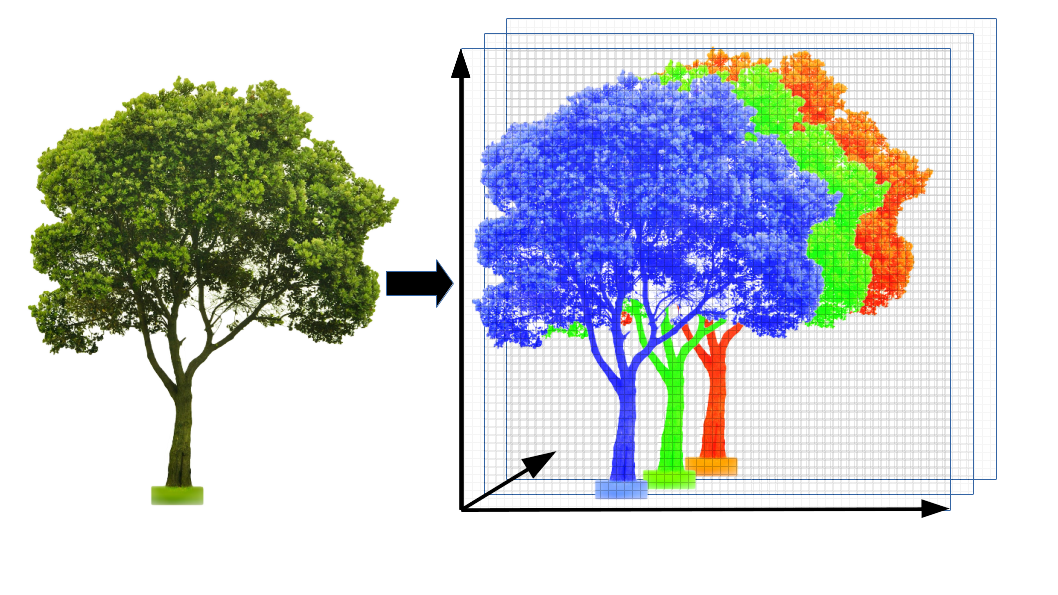
\includegraphics[width=\linewidth]{../graphs/tree/full}
 \captionsetup{width=0.8\linewidth, font=small}
 \captionof{figure}{An image of a tree, split into the three color channels.}
\end{Figure}
\noindent When convolving over such a picture using 2D-convolution, one can apply a series of two-dimensional filters, i.e. filters of a certain height and width.\\
This is however not the case with the CullPDB data. Our dataset is essentially one-dimensional, with a breadth of 700 amino acids, but instead of 3 color channels, it contains 57 features ("channels").
\begin{Figure}
 \centering
 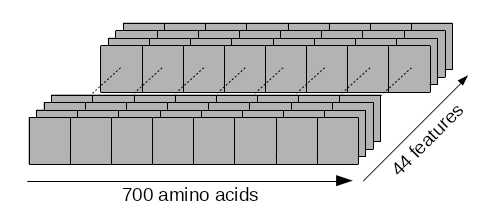
\includegraphics[width=\linewidth]{../graphs/tree/amino}
 \captionsetup{width=0.8\linewidth, font=small}
 \captionof{figure}{The input part of the dataset used in our models.}
\end{Figure}
\noindent Of these 57 features, we will be using the first 22 (amino acid residues) as well as the final 22 (the amino acid sequence profile) as input data, while in the end supplying an output of still 700 amino acids, but with 9 or 2 (secondary structures / solvent accessibility) channels for the single-task models and 11 (both) channels in the multi-task model.


\subsection{Tools}
\subsubsection{Model}
Being that we are training a convolutional neural network, in particular two sets of functions are important, namely activation and loss functions.

The activation functions we opted to use in this project were the rectifier, softmax and sigmoid functions respectively, whereas we use the Cross Entropy loss in evaluating and training the network.
\paragraph{Rectifier}
Possibly the simplest of these activation functions is the rectifier, which when implemented in an artificial neural network is referred to as a \textit{rectified linear unit} (ReLU), which, in laymans terms, simply does not allow negative values, and replaces such values with zero.
\[
ReLU(x) = x^+ = max(0,x)
\]

\paragraph{Sigmoid function}
Sigmoid functions are a specific variant of logistic functions, and serve to map values in arbitrary ranges to values within a specific range, so that the mapped values over the original values form a sigmoid curve. The value of applying sigmoid functions to outputs from a neural network is that they then enable the model to map its output of arbitrarily big or small values to a probability (i.e. a value $0\leq x \leq 1$). In the present case, this becomes relevant when predicting relative and absolute solvent accessibilities.
\[
Sigmoid(x) = \frac{1}{1 + e^{-x}} = \frac{e^x}{e^x +1}
\]

\begin{Figure}
 \centering
 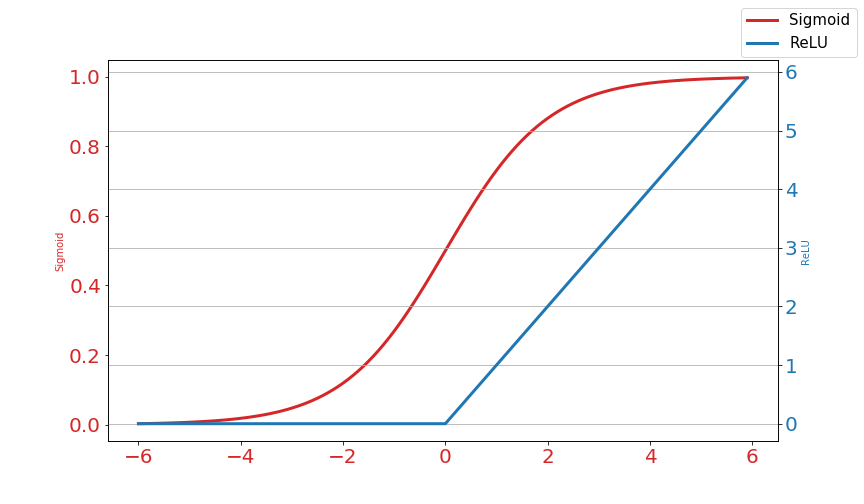
\includegraphics[width=\linewidth]{../graphs/activation.png}
 \captionsetup{width=0.8\linewidth, font=small}
 \captionof{figure}{The sigmoid and rectifier activation functions}
\end{Figure}

%\begin{wrapfigure}{I}{\linewidth}
%\centering
%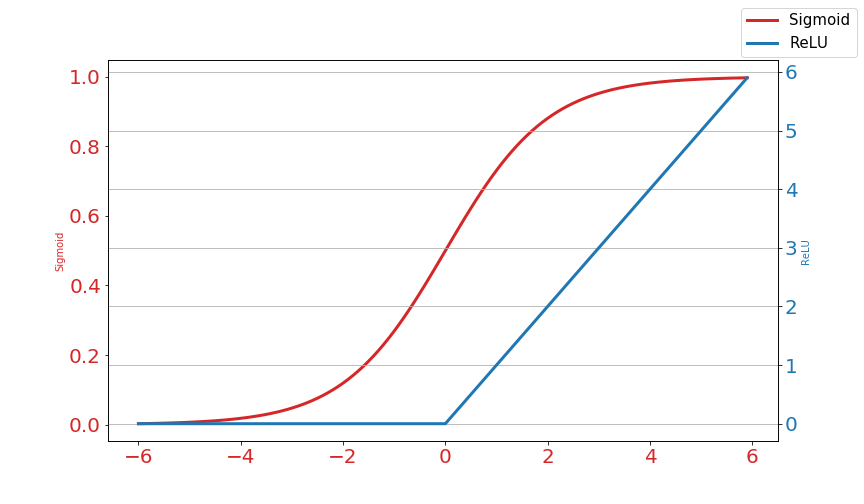
\includegraphics[width=\linewidth]{../graphs/activation.png}
%\caption{This is the former Share\LaTeX{} logo}
%\end{wrapfigure}

%\begin{figure}[h]
%  \centering
%  \frame{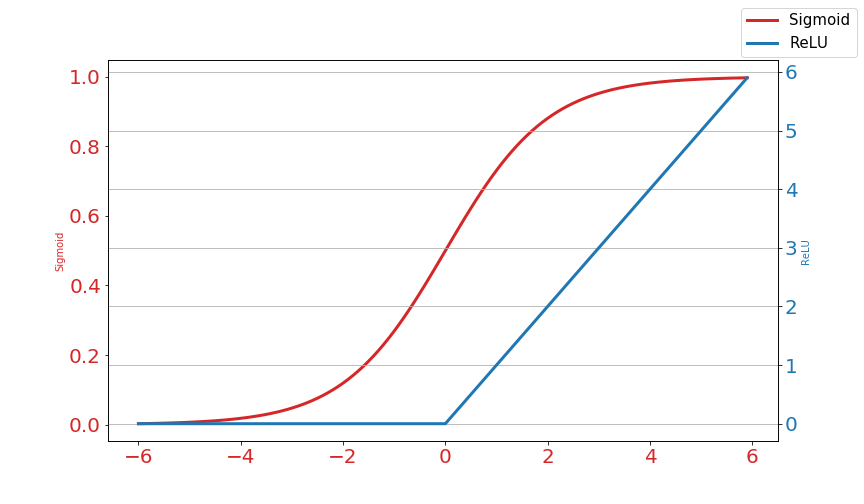
\includegraphics[width=\textwidth]{../graphs/activation}}
%  \caption{The sigmoid and rectifier activation functions}
%\end{figure}

\paragraph{Softmax}
The softmax function ($\sigma$) does very much the same as the sigmoid, only for a range of values. In other words, a set of non-normalized values (that is: of arbitrary length and spread) can via softmax be mapped to a probability distribution over that set. This means that all the values $x_i$ are in the range $0\leq x_i \leq 1$, and that they sum to 1.

This is especially relevant in cases where one is attempting to perform classification, such as which is the present case where we are training the model to predict amino acid secondary structures. 

Applying a softmax function on a dataset \textit{x} of \textit{j} elements would be as follows:
$$
\sigma(x_i) = \frac{e^{x_i}}{\sum_{j=1} e^{x_j}}
$$

\begin{Figure}
 \centering
 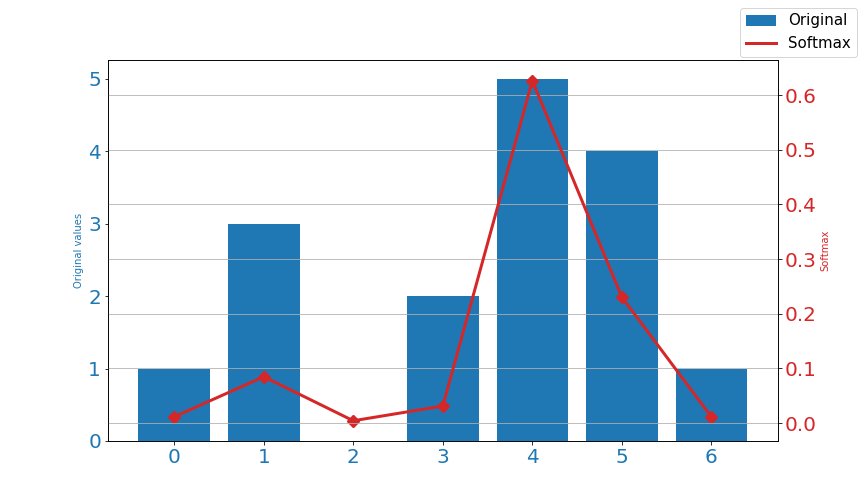
\includegraphics[width=\linewidth]{../graphs/softmax}
 \captionsetup{width=0.8\linewidth, font=small}
 \captionof{figure}{Example data softmaxed}
\end{Figure}
One will often see a very similar function called the \textit{Logarithmic Softmax} which resembles the above, but with the addition that the probability $\sigma(x_i)$ equals the natural logarithm of the same:
\[
\sigma_{log}\left(x_{i}\right)=\log \left(\frac{e^{ x_{i}}}{\sum_{j=1} e^{ x_{j}}}\right)
\]
In practical implementations this approach helps preventing possible underflows.

%\begin{figure}[h]
%  \centering
%  \frame{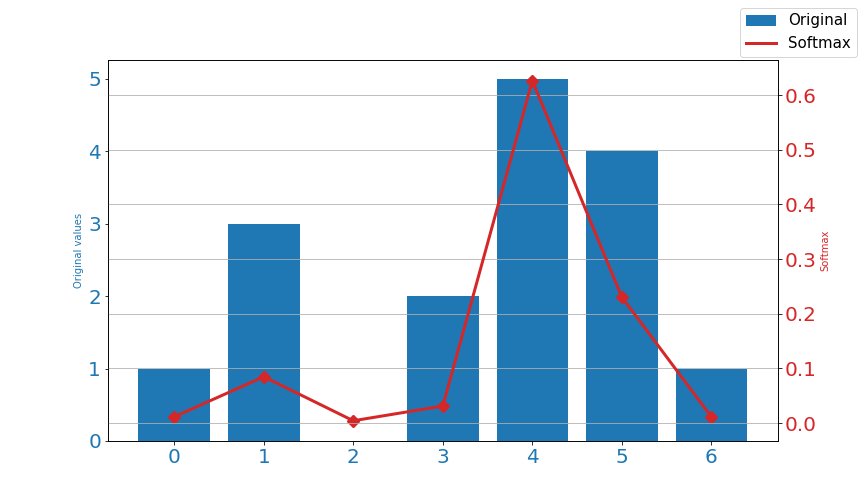
\includegraphics[width=\linewidth]{../graphs/softmax}}
%  \caption{Example data softmaxed}
%\end{figure}


\paragraph{Cross Entropy Loss}
Between two probability distributions each over the same set of outcomes there exists a certain cross entropy.
Thus, given two probability distributions \textit{m} and \textit{n} predicting the discrete outcome $\mathcal{Z}$, the formula for calculating the cross entropy is:
$$L ( m , n ) = - \sum _ { z \in \mathcal { Z } } m ( z ) \log n ( z )$$
A specific instance of the cross entropy loss is the \textit{binary cross entropy loss}, which is useful in cases where the possible outcome is binary (i.e. there are only two possible outcomes). 
\\
Seing as the aim of this paper was to train our network to perform classifications first on amino acid secondary structures (of which there are eight) and then relative and absolute solvent accessibility (which are both encoded as either ones or zeros), we have used a Cross Entropy Loss function on the former and a Binary Cross Entropy Loss function on the two latter.


\paragraph{Optimization algorithm}
Several choices exist for the choice of optimization algorithm. One simple algorithm would be Stochastic gradient descent, in which there is one learning rate that applies to all model parameters (weights) and does not change throughout training.\\
Other optimizations such as Adabtive Gradient Algorithm (AdaGrad) maintains a learning rate for each parameter in the model, while algorithms such as the Root Mean Square Propagation (RMSProp) algorithm continuously adjusts the learning rate in accordance to the average magnitude in recent gradients.\\
In this project we have opted to use the Adam optimizer, introduced by \citeauthor{Adam} no more than four years ago. This optimizer combines two of the above aspects, namely individual learning rates for each parameter and continous evaluation of the learning rates. However while RMSProp only evaluates the learning rate in response to the mean magnitude of gradients, Adam also evaluates on the variance of recent gradients.\\
To do this, \citeauthor{Adam} writes that the Adam optimizer has four configuration parameters: 
\begin{itemize}
\item $\alpha$: The initial learning rate,
\item $\beta_1$: The exponential decay rate for the mean of gradients
\item $\beta_2$: The exponential decay rate for the variance of gradients
\item $\epsilon$: A very small value useful to prevent division by zero
\end{itemize}
In the section 'Which optimizer to use?' of his 2016 article "An overview of gradient descent optimization algorithms" author \citeauthor{Ruder16} writes:

\textit{"Insofar, RMSprop, Adadelta, and Adam are very similar algorithms that do well in similar circumstances. \citeauthor{Adam} show its bias-correction helps Adam slightly outperform RMSprop towards the end of optimization as gradients become sparser. Insofar, Adam might be the best overall choice."}\\
In this project we have chosen to follow the advice of \citeauthor{Ruder16} and use the Adam optimization algorithm.

\subsubsection{Technological implementation details}
In training our network we utilized a machine learning framework for Python called \href{https://pytorch.org/}{PyTorch}, specifically optimized for building deep neural networks. \\
The PyTorch library is build upon the \href{http://torch.ch/}{Torch} library, originally a machine learning library and language based on the scripting language Lua.\\
The strength in using PyTorch stems from several aspects:
\paragraph{GPU support}
PyTorch provides a strong framework for performing calculations on a graphical processing unit rather than the computer's CPU. While GPUs are valued in video game circles, they are also enourmously useful for performing machine learning, since this is often tasks that involve a high number of calculations that can perfectly fine be performed in parallel. For this, a GPU is preferred over a CPU since they often have a much higher number of cores, and are thus better suited for parallel programming. Indeed in our case, there was a factor of 20 difference in the time needed to train an epoch between doing it on the CPU versus the GPU.
\paragraph{Tensors}
The main data structure used in the PyTorch framework is tensors. Where a vector is a 1-dimensional array and a matrix a 2-dimensional array, a tensor is a multi-dimensional array. This means they can be 1-, 2-, 3- or even 42-dimensional arrays. As such tensors subsume scalars, vectors and matrices. (KILDE ER DEEPLEARNING BOGEN p 211). Tensors in PyTorch are multi-dimensional arrays much like the ones implemented in numpy, but with the option to place it on the GPU rather than the CPU.
\paragraph{Automatic differentiation}
In order to utilize the backpropagation that lets neural networks train and improve, the loss must be differentiated in regards to all of the weights and values in the model in order to calculate the gradients. This can be a cumbersome task when performed by hand, but PyTorch provides a powerful tool in for of the \texttt{autograd} and \texttt{optim} modules. The first of these modules keeps track of which computations were performed on which variables in order to arrive at the final value of a variable, so that it can be retraced backwards in the end to calculate gradients, while the latter contains ready-made implementations of several optimization algorithms (among them Adam), which automatically adjusts the weights and values in the model, according to the calculated gradient and a supplied learning rate.\\
These things combined allow a training step for a neural network to be performed in as few steps as shown below:
\begin{lstlisting}
# Setup
LR = 0.0025              # learning rate
optimizer = torch.optim.Adam(cnn.parameters(), lr=LR)
loss_func = nn.CrossEntropyLoss()

# One training step
output = cnn(b_x)
loss = loss_func(output, b_y)
optimizer.zero_grad()
loss.backward()
optimizer.step()
\end{lstlisting}

\paragraph{Ready-made implementations}
A final helpful aspect of using PyTorch for implementing artificial neural networks is the abundance of already implemented algorithms and functions. This adds the further detail to the implementation that several of the most often used functions have been written together for reasons of numerical stability. 

For example, the above mentioned Cross Entropy Loss function, which when implemented in PyTorch also contains an implementation of the \texttt{LogSoftmax()} function. The documentation for PyTorch reveals that the implementation then becomes:

\begin{align*}
\operatorname{loss}(x, \text {class})&=-\log \left(\frac{e^{ x[\text {class}]}}{\sum_{j} e^{ x[j]}}\right)\\
&=-x[\text {class}]+\log \left(\sum_{j} e^{x[j]}\right)
\end{align*}

\noindent A similar circumstance is that of the Binary Cross Entropy loss, where PyTorch provides an implementation in the form of \texttt{BCEWithLogitsLoss()} which readily combines the Binary Cross Entropy Loss with a sigmoid function, again in order to provide numerical stability. In this case the implementation becomes: \\
\[
\ell(m, n)=L=\left\{l_{1}, \ldots, l_{N}\right\}^{\top}
\]
where
\[ \quad l_{n}=-w_{n}\left[n_{n} \cdot \log m_{n}+\left(1-n_{n}\right) \cdot \log \left(1-m_{n}\right)\right]
\]

\subsubsection{Hardware}
In terms of performing the calculations, all of our training of the model was done on a Dell PC with a 7th gen octocore Intel Core i7 CPU, 16GB of RAM and a Nvidia GeForce GTX 1050TI GPU with 4GB of RAM and 768 cores running Linux.

\subsection{Single-task secondary structure prediction}
We built a convolutional neural network, implemented in Python using PyTorch in order to predict amino acid secondary structures from the amino acid residues as well as the sequence profile. We tested variations on number of layers, layer depth, kernel sizes and learning rate (results below) in order to maximize performance of the model. 

\subsubsection{Architecture}

The basic structure of the model remained unchanged throughout these test. The basics of the structure was comprised of following elements:
\begin{itemize}
\item It was to be a deep neural network (i.e. at least one hidden layer of neurons),
\item The layer debth was to remain the same throughout the network,
\item Sufficient padding was to be added to the convolving layers so that the breadth of the intermediary values remained the same (the 700 amino acids, that is),
\item After each layer, save the last, the layer was activated using a rectified linear unit,
\item The model should not itself contain a SoftMaxing layer, since this was built into the loss function,
\item The model was evaluated and optimized based on the output of a Cross Entropy loss function,
\item The model was to be optimized based on the loss on the training set while being continuously humanly evaluated on the loss and accuracy on the validation set.
\end{itemize}

\begin{Figure}
 \centering
 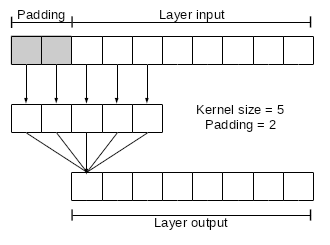
\includegraphics[width=\linewidth]{../graphs/padding}
 \captionsetup{width=0.8\linewidth, font=small}
 \captionof{figure}{The layer breadth is preserved across convolutions thanks to padding.}
\end{Figure}

\subsubsection{Accuracy}
Having built a network that was training and improving on the training set data, it was also relevant evaluate the accuracy of the predictions of the network in addition to the calculation of loss on the validation set.

Several approaches to evaluating predictions exist. The output of our model was something of a proxy to a probability distribution, however not a true probability distribution since the model itself did not perform a SoftMax on the output. This was however not an issue, since the index of the largest value in a set of values remains the same before and after being SoftMaxed, and we could thus safely treat the index of the largest value in the un-SoftMaxed output as the label of the prediction.

In implementing a procedure to evaluate the accuracy of a prediction, we first collapse the output distribution as just described, and then produce a matrix of indicators as to whether the predicted label matched the label in the matrix of actual secondary structure labels as provided by the database.

Of course at this point the model would also be evaluated on its accurate prediction of padding (a task that proved remarkably managable), and thus could achieve arbitrarily high accuracy just by adding more padding to the set. To avoid this, we construct a masking matrix from the values in the target set that are \texttt{NoSeq}. We can then use this mask to filter out the irrelevant values in our matrix of correct and false predictions.

Finally taking the mean of this, now filtered, matrix of prediction correctness produces the percentage of the relevant predictions that were in fact correct.
\begin{Figure}
 \centering
 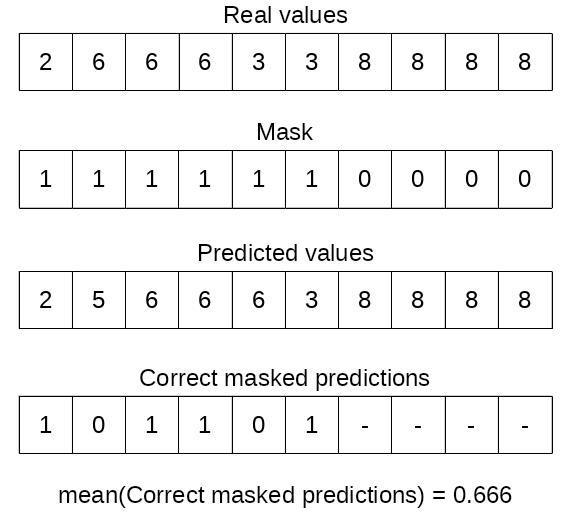
\includegraphics[width=0.8\linewidth]{../graphs/accuracy}
 \captionsetup{width=0.8\linewidth, font=small}
 \captionof{figure}{Calculating accuracy.}
\end{Figure}

\subsection{Single-task solvent accessibility prediction}
For comparison purposes, we also implemented a convolutional neural network to predict the two solvent accessibility features alone. This model is in most regards similar to the above, only with fewer output-channels and different final activation and loss functions.\\
One could think of the types of these three (structures, relative and absolute solvency) output as identical; the structure labels are a probability distribution while in a certain sense so are the solvent accessibility features - only a probability between two possible outcomes.\\
Nonetheless different final activation function were needed for the two latter, since performing a softmax on the binary output would always yield a 1. Thus the two solvent features are activated by a sigmoid function - effectively mapping their value to a probability between 0 and 1. Further, the loss function, now only distinguishing between two possible classes (0 and 1) should be the Binary Cross Entropy.\\
rom a technical implementational perspective, as how in the previous model the SoftMax function was already included in the PyTorch implementation of BCELoss, in this case the sigmoid function is not explicitly stated in the model, as it is already included in the PyTorch module \texttt{BCEWithLogitsLoss} - the Binary Cross Entropy loss function.

\subsection{Multi-task learning}
%\subsubsection{Generelt om Multi-task learning}
There are multiple ways of implementing multi-task learning in artificial neural networks. The most basic distinction is between implementing the network using soft or hard parameter sharing. In the case of hard parameter sharing, the input data gets transformed through a number of layers in its entirety only then to be split into distinguishable output sets, and then optionally go through further set-specific layers. This approach provides a very strong line of defence against overfitting, as forcing the model to optimize on several predictive capabilities makes it less  susceptible to representing the aspects of the training data that are not representative of general tendencies in the domain. 

In contrast to this stands soft parameter sharing, in which one could say that the model is comprised of a series of sub-models, each containing their own distinct layers and oriented towards each their prediction task. In this case the parameters of each of the models are balanced and regularized against each other in order to make them as similar as possible.

On the grounds that the data set we are working with is somewhat limited (5926 proteins out of some 400.000 in the original PDB database) we were concerned about possible overfitting, and thus opted to implement our multi-task learning network with hard parameter sharing.

\subsubsection{Architecture}
Having decided on employing hard parameter sharing, we implemented the model in much a similar fashion to the single-task model explained above (i.e. convolutional layers, ReLU, padding, etc.). What sets the two models apart is the fact that in the final layer of the multi-task model the data is split up into the three output sets, secondary structure and relative/absolute solvent accessibility.\\
\\

\begin{Figure}
 \centering
 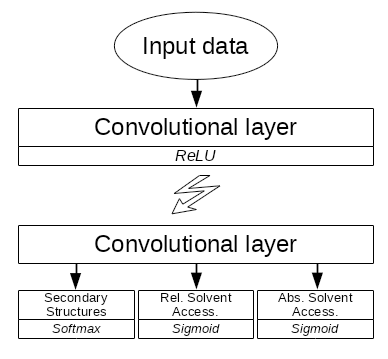
\includegraphics[width=\linewidth]{../graphs/arch}
 \captionsetup{width=0.8\linewidth, font=small}
 \captionof{figure}{Model architecture: The lightning represents one or more similar convolutional layers.}
\end{Figure}

\subsubsection{Training}
Utilizing the PyTorch loss function, autogradient and optimizer-libraries, implementing a model with essentially three losses is easy. As mentioned above, the model had a Cross Entropy loss for the secondary structure prediction, as well as two Binary Cross Entropy losses for the two solvency features. Training the model with regards to minimizing these losses is acheived simply by letting a variable be the sum of the three, and then letting the library automatically backtrace each of the parameters in the model via this value.
\begin{lstlisting}
# Calculate losses
loss1 = loss_func_structure(calc_struct,  correct_struct)
loss2 = loss_func_solvent(calc_rel, correct_rel)
loss3 = loss_func_solvent(calc_abs,  correct_abs)

# Sum the losses
loss_sum = (loss1 + loss2 + loss3)

# Backpropagate and train
loss_sum.backward()
optimizer.step()
\end{lstlisting}


\subsubsection{Accuracy}
Evaluating the accuracy of the model's predictions happens for each of the three features being predicted in the model.\\
The accuracy of the secondary structure label prediction happens in a similar fashion to the one in the single-task model. Seing as we know the structure of the solvent accessibility features to be binary and independent (an amino acid can be relatively solvent while not absolutely solvent and vica-versa), we can, after manually applying a sigmoid function on them, employ a simple round function to convert the probability outputted by the model to a binary prediction.\\
Having done so, the same method of constructing a matrix of correct and false predictions and then filtering this matrix by the mask already derived from the secondary structures was used.


\subsection{Hyperparameters}
In order to optimize our two models we iterated over a series of values for the models' hyperparameters, that is the number of layers, the depth of the layers, the learning rate and the size of the kernels used in the convolutions.\\
For a starting point, we chose to adapt the values used by Xi et. al, and then iterated to both sides of those values.\\
An initial decision to make was the batch size - that is how many inputs from the data set to process at once. In general there are three approaches how many data points to train on at once, compared to the total length of the data (LOD):
\begin{center}
\begin{tabular}{l|c}
\hline 
Name & Size \\ 
\hline 
Batch gradient & Size = LOD \\ 

Minibatch gradient & 1 $<$ Size $<$ LOD \\ 

Generative Stochastic & 1 \\ 
\hline 
\end{tabular} 
\end{center}
In the case of Generative Stochastic networks, the model is continuously trained on random single data points, and is generally accepted to produce better predictions than both batch and mini-batch gradient descents, however at the cost of increased training time.
Batch gradient was not an option for us, for the simple practical reason that there was not enough memory on our GPU to handle the entire data set at once. We opted for a batch size of 4 throughout our tests in a compromise between predictive power and speed of training.
A test of accuracy over different batch sizes can be found in the appendix.











\end{multicols}
\section{Results}
In our optimization of the model we iterated over the hyperparemeters in the order: No. of layers, learning rate, debth of layers and kernel size. For each hyperparameter we adjusted the value and allowed the multi-task model to train for 10 epochs and then evaluate accuracy of both the Q8 secondary structure prediction as well as the relative and absolute solvent accessibiliy on both the validation and test set.\\
In choosing which values to continue with for the final model we only considered results on the validation set, and attempted to balance accuracy with model size and trainability.\\
Once we had found what configurations performed the best on the respective parameters, we trained both our single- and multi-task models with these parameters for 20 epochs and compared the results.

\subsection{Hyperparameters}
\subsubsection{No. of layers}
Variying the number of layers in the model greatly affects the size of the model and thus also the time taken to train it. Further, adding more layers increases the risk of overfitting (factcheck lige det...).\\
In our tests we evaluated from two to five hidden layers. Note, that the output layer is not counted in this number.

% Please add the following required packages to your document preamble:
% \usepackage[normalem]{ulem}
% \useunder{\uline}{\ul}{}
\begin{table}[H]
\centering
\begin{tabular}{lcccccc}
\multicolumn{7}{c}{\textbf{No. of layers}} \\
\multicolumn{7}{c}{\textit{Layer debth = 80, kernel size = 11, learning rate = 0.00025, batch size = 4}} \\ \hline
\multicolumn{1}{l|}{} & \multicolumn{3}{c|}{{\ul Validation set}} & \multicolumn{3}{c}{{\ul Test set}} \\
\multicolumn{1}{c|}{Layers} & Q8 & \begin{tabular}[c]{@{}c@{}}Relative\\ solvent\\ accessibility\end{tabular} & \multicolumn{1}{c|}{\begin{tabular}[c]{@{}c@{}}Absolute\\ solvent\\ accessibility\end{tabular}} & Q8 & \begin{tabular}[c]{@{}c@{}}Relative\\ solvent\\ accessibility\end{tabular} & \begin{tabular}[c]{@{}c@{}}Absolute\\ solvent\\ accessibility\end{tabular} \\ \hline
\multicolumn{1}{l|}{2} & 69.79\% & 81.94\% & \multicolumn{1}{c|}{80.58\%} & 69.783\% & 82.001\% & 80.413\% \\
\multicolumn{1}{l|}{3} & 70.08\% & 82.69\% & \multicolumn{1}{c|}{81.10\%} & 70.447\% & 82.259\% & 80.701\% \\
\multicolumn{1}{l|}{4} & 70.11\% & 82.90\% & \multicolumn{1}{c|}{81.18\%} & 70.143\% & 82.291\% & 80.528\% \\
\multicolumn{1}{l|}{5} & 69.48\% & 82.73\% & \multicolumn{1}{c|}{81.13\%} & 69.343\% & 82.158\% & 80.365\% \\
\multicolumn{1}{l|}{16} & 68.15\% & 82.15\% & \multicolumn{1}{c|}{80.42\%} & 68.459\% & 81.595\% & 79.924\% \\
\multicolumn{1}{l|}{32} & 66.94\% & 81.61\% & \multicolumn{1}{c|}{79.85\%} & 67.279\% & 81.196\% & 79.483\% \\
\multicolumn{1}{l|}{64} & 65.10\% & 80.97\% & \multicolumn{1}{c|}{79.25\%} & 65.100\% & 80.644\% & 78.899\%
\end{tabular}
\end{table}
\noindent We made the dicision after this test to continue with 3 hidden layers, as we did not feel that the gained accuracy by advancing to 4 matched the increased cost of training the network.


\subsubsection{Learning rate}
Having a bad learning rate puts the model in risk of several things. A learning rate too small will possibly trap the model in a local minimum, whereas a learning rate too big will risk not being able to hit global maxima, but constantly shifting around them. Further, a lower learning rate means more time needed to train, while a larger learning rate might in the worst case actually miss a global maximum.\\
Below are the results of our tests of learning rate.
% Please add the following required packages to your document preamble:
% \usepackage[normalem]{ulem}
% \useunder{\uline}{\ul}{}
\begin{table}[H]
\centering
\begin{tabular}{lcccccc}
\multicolumn{7}{c}{\textbf{Learning rate}} \\
\multicolumn{7}{c}{\textit{Layer debth = 80, kernel size = 11, 3 hidden layers, batch size = 4}} \\ \hline
\multicolumn{1}{l|}{} & \multicolumn{3}{c|}{{\ul Validation set}} & \multicolumn{3}{c}{{\ul Test set}} \\
\multicolumn{1}{c|}{\begin{tabular}[c]{@{}c@{}}Learning\\ rate\end{tabular}} & Q8 & \begin{tabular}[c]{@{}c@{}}Relative\\ solvent\\ accessibility\end{tabular} & \multicolumn{1}{c|}{\begin{tabular}[c]{@{}c@{}}Absolute\\ solvent\\ accessibility\end{tabular}} & Q8 & \begin{tabular}[c]{@{}c@{}}Relative\\ solvent\\ accessibility\end{tabular} & \begin{tabular}[c]{@{}c@{}}Absolute\\ solvent\\ accessibility\end{tabular} \\ \hline
\multicolumn{1}{l|}{0.00005} & 66.85\% & 81.61\% & \multicolumn{1}{c|}{79.89\%} & 66.958\% & 81.052\% & 79.490\% \\
\multicolumn{1}{l|}{0.0001} & 68.71\% & 82.18\% & \multicolumn{1}{c|}{80.42\%} & 68.983\% & 81.737\% & 80.042\% \\
\multicolumn{1}{l|}{0.00025} & 70.38\% & 82.78\% & \multicolumn{1}{c|}{81.23\%} & 70.386\% & 82.077\% & 80.576\% \\
\multicolumn{1}{l|}{0.0005} & 70.83\% & 82.86\% & \multicolumn{1}{c|}{81.13\%} & 70.624\% & 82.136\% & 80.437\% \\
\multicolumn{1}{l|}{0.001} & 70.66\% & 82.75\% & \multicolumn{1}{c|}{80.92\%} & 70.287\% & 82.040\% & 80.426\% \\
\multicolumn{1}{l|}{0.0025} & 69.12\% & 81.67\% & \multicolumn{1}{c|}{79.59\%} & 68.590\% & 81.294\% & 79.806\%
\end{tabular}
\end{table}
Not only did the non-optimal learning rates not perform as well as 0.0005, but they also trained significantly slower, as seen on the graph below.
\begin{figure}[H]
  \centering
  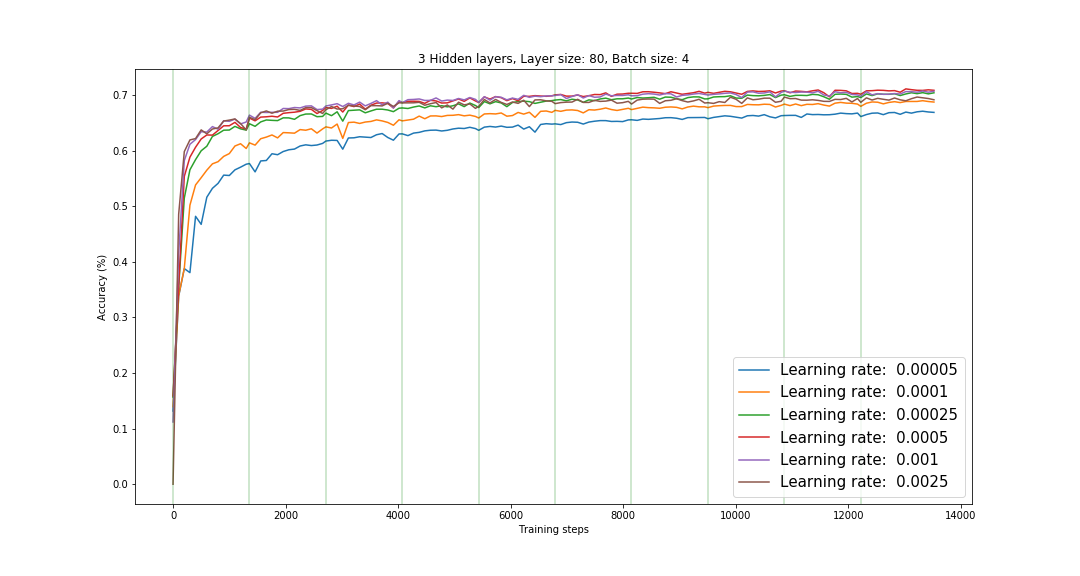
\includegraphics[width=\linewidth]{../graphs/new/learning_rate}
  \caption{Accuracy on the validation with varying learning rate. The green lines represent epochs.}
\end{figure}
For the remainder of the tests we used a learning rate of 0.0005.

\subsubsection{Depth of layers}
As with the number of layers, the depth affects both model potential complex predictive performance and model weight and size. We started from the depth of 100 as also used by Xi et al. and found that no increase in performance was acheived by adding more depth, however some gains were made by shallowing down the layers a bit.

\begin{table}[H]
\centering
\begin{tabular}{lcccccc}
\multicolumn{7}{c}{\textbf{Layer depth}} \\
\multicolumn{7}{c}{\textit{Learning rate = 0.0005, kernel size = 11, 3 hidden layers, batch size = 4}} \\ \hline
\multicolumn{1}{l|}{} & \multicolumn{3}{c|}{{\ul Validation set}} & \multicolumn{3}{c}{{\ul Test set}} \\
\multicolumn{1}{c|}{Depth} & Q8 & \begin{tabular}[c]{@{}c@{}}Relative\\ solvent\\ accessibility\end{tabular} & \multicolumn{1}{c|}{\begin{tabular}[c]{@{}c@{}}Absolute\\ solvent\\ accessibility\end{tabular}} & Q8 & \begin{tabular}[c]{@{}c@{}}Relative\\ solvent\\ accessibility\end{tabular} & \begin{tabular}[c]{@{}c@{}}Absolute\\ solvent\\ accessibility\end{tabular} \\ \hline
\multicolumn{1}{l|}{50} & 70.14\% & 81.94\% & \multicolumn{1}{c|}{81.07\%} & 70.436\% & 82.280\% & 80.395\% \\
\multicolumn{1}{l|}{60} & 70.77\% & 82.68\% & \multicolumn{1}{c|}{81.17\%} & 70.407\% & 81.931\% & 80.295\% \\
\multicolumn{1}{l|}{70} & 70.03\% & 82.97\% & \multicolumn{1}{c|}{81.20\%} & 70.931\% & 82.392\% & 80.723\% \\
\multicolumn{1}{l|}{80} & 70.86\% & 82.78\% & \multicolumn{1}{c|}{81.14\%} & 70.881\% & 82.228\% & 80.535\% \\
\multicolumn{1}{l|}{90} & 71.19\% & 83.09\% & \multicolumn{1}{c|}{81.37\%} & 70.973\% & 82.472\% & 80.734\% \\
\multicolumn{1}{l|}{100} & 70.95\% & 82.05\% & \multicolumn{1}{c|}{80.31\%} & 71.007\% & 82.704\% & 80.602\%
\end{tabular}
\end{table}
\noindent As is seen in the table a depth of 90 filters proved most accurate on our tests. Below is shown a graph of three of the values, illustrating how a depth of 90 performed better than the two other continuously throughout training. Refer to the appendix for at graph containing all the tested  depths.
\begin{figure}[H]
  \centering
  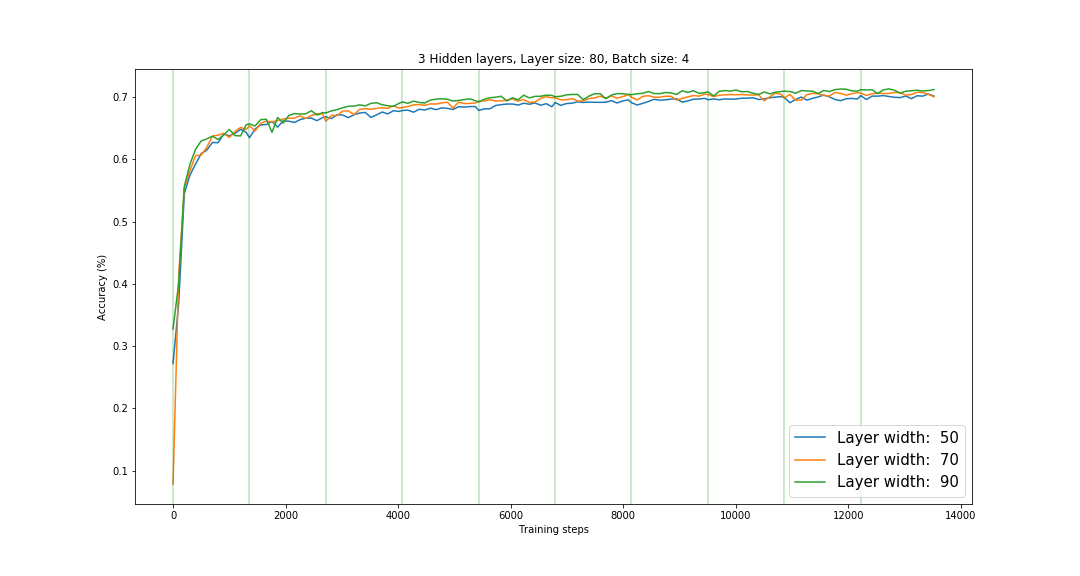
\includegraphics[width=\linewidth]{../graphs/new/layer_width_1}
  \caption{Accuracy on the validation set with varying layer depth.}
\end{figure}
\subsubsection{Kernel size}
Fortæl om kernel sizes og om hvordan vi først prøvede én størrelse på dem alle og siden at variere størrelsen (lav evt. en reference til nogen af dem der har trænet på MNIST og deres kernel sizes), lav en tabel og to grafer.

In the article by Xi et al, a kernel size of 11 was chosen on the basis that the average length of an $\alpha$-helix chain, and in accordance with this we tested values in the vicinity. For the sake of padding we stuck to uneven values.\\
While the first tests fokus on keeping the same size of kernel throughout the layers in the model, we also performed a series of tests using increasing, decreasing, pyramid-shaped and valley-shaped progressions of kernel sizes.

% Please add the following required packages to your document preamble:
% \usepackage[normalem]{ulem}
% \useunder{\uline}{\ul}{}
\begin{table}[H]
\centering
\begin{tabular}{ccccccc}
\multicolumn{7}{c}{\textbf{Kernel sizes}} \\
\multicolumn{7}{c}{\textit{Learning rate = 0.0005, layer depth = 90, 3 hidden layers, batch size = 4}} \\ \hline
\multicolumn{1}{l|}{} & \multicolumn{3}{c|}{{\ul Validation set}} & \multicolumn{3}{c}{{\ul Test set}} \\
\multicolumn{1}{c|}{\begin{tabular}[c]{@{}c@{}}Kernel\\ Size\end{tabular}} & Q8 & \begin{tabular}[c]{@{}c@{}}Relative\\ solvent\\ accessibility\end{tabular} & \multicolumn{1}{c|}{\begin{tabular}[c]{@{}c@{}}Absolute\\ solvent\\ accessibility\end{tabular}} & Q8 & \begin{tabular}[c]{@{}c@{}}Relative\\ solvent\\ accessibility\end{tabular} & \begin{tabular}[c]{@{}c@{}}Absolute\\ solvent\\ accessibility\end{tabular} \\ \hline
\multicolumn{1}{c|}{5} & 71.00\% & 82.54\% & \multicolumn{1}{c|}{81.20\%} & 70.455\% & 82.405\% & 80.657\% \\
\multicolumn{1}{c|}{7} & 71.50\% & 82.24\% & \multicolumn{1}{c|}{81.00\%} & 71.616\% & 82.241\% & 80.611\% \\
\multicolumn{1}{c|}{9} & 71.44\% & 82.95\% & \multicolumn{1}{c|}{81.24\%} & 71.409\% & 82.363\% & 80.714\% \\
\multicolumn{1}{c|}{11} & 70.94\% & 82.15\% & \multicolumn{1}{c|}{80.52\%} & 70.957\% & 82.592\% & 80.742\% \\
\multicolumn{1}{c|}{13} & 70.82\% & 82.49\% & \multicolumn{1}{c|}{80.97\%} & 70.903\% & 82.389\% & 80.605\% \\ \hline
\multicolumn{1}{c|}{{[}5,7,9,11{]}} & 71.55\% & 82.98\% & \multicolumn{1}{c|}{81.48\%} & 71.636\% & 82.525\% & 80.963\% \\
\multicolumn{1}{c|}{{[}7,9,11,13{]}} & 71.17\% & 82.75\% & \multicolumn{1}{c|}{81.20\%} & 71.284\% & 82.778\% & 80.856\% \\
\multicolumn{1}{c|}{{[}11,9,7,5{]}} & 71.21\% & 82.43\% & \multicolumn{1}{c|}{81.00\%} & 71.387\% & 82.221\% & 80.712\% \\
\multicolumn{1}{c|}{{[}7,9,9,7{]}} & 70.78\% & 82.88\% & \multicolumn{1}{c|}{81.34\%} & 71.588\% & 82.673\% & 80.956\% \\
\multicolumn{1}{c|}{{[}9,7,7,9{]}} & 71.20\% & 82.87\% & \multicolumn{1}{c|}{81.26\%} & 71.424\% & 82.365\% & 80.845\%
\end{tabular}
\end{table}
\begin{figure}[H]
  \centering
  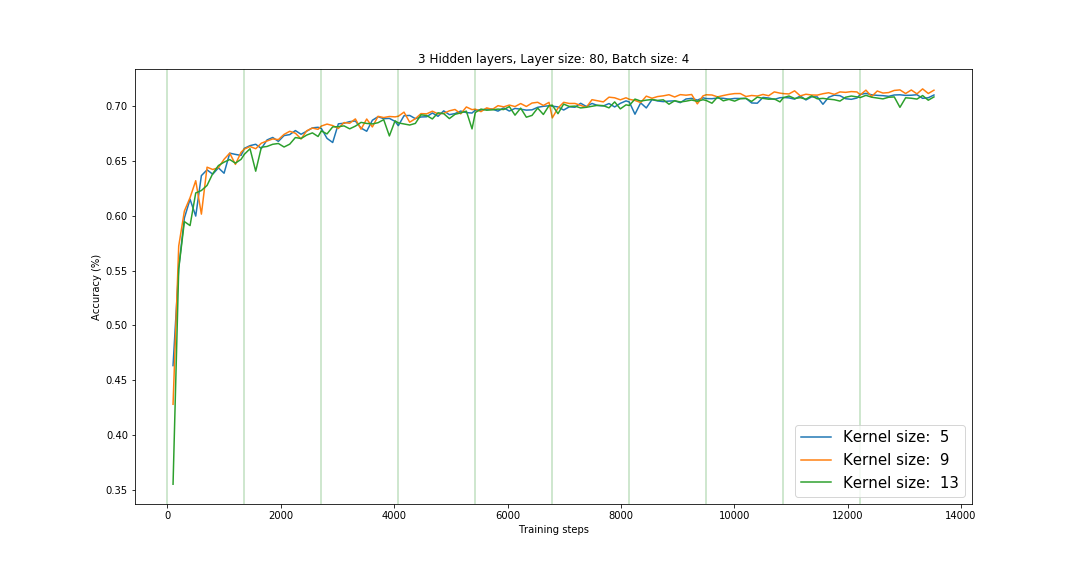
\includegraphics[width=\linewidth]{../graphs/new/kernel_sizes_2}
  \caption{Constant kernel size.}
\end{figure}

\begin{figure}[H]
  \centering
  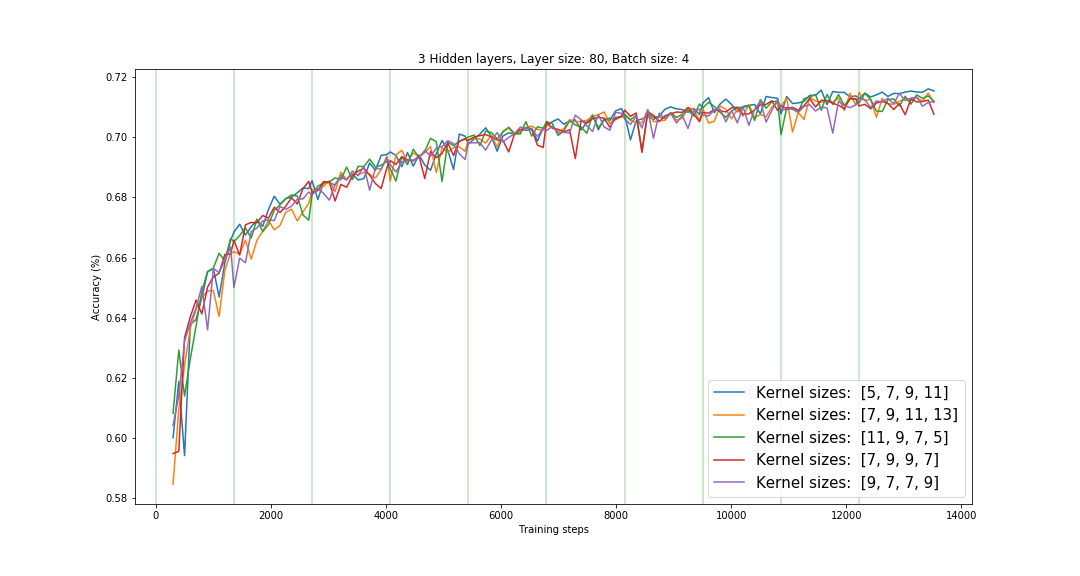
\includegraphics[width=\linewidth]{../graphs/new/kernel_sizes_1}
  \caption{Varying kernel size.}
\end{figure}

\noindent As with the layer depth, not all values are shown in the graph - refer to the appendix for a graph with all values.\\
It became clear that using a progressively rising size of kernels a significant increase was seen in accuracy. For the final model we opted to use kernel sizes [5, 7, 9, 11].\\
What is interesting about the data shown above, is that while one would expect larger kernel sizes to increase performance, or at the very least not decrease it (since the model should learn just to 'ignore' extra space in the kernel), the model's performance did indeed decrease as the kernel sizes grew.



\subsection{Final predictive capabilities}
\textit{Forklar hvordan vi fandt frem til vores hyperparametre på multi-task modellen og så anvendte de samme på single-task. Skriv noget tekst om hvordan vi på test-sættet nåede op på so-and-so meget præcision på hhv. den ene og anden model og hhv. strukturer og solvent egenskaber, samt sammeligning af resultatet på test- og valideringssæt.}

Having performed the series of tests described above we settled on the following architecture:
\begin{table}[H]
\centering
\begin{tabular}{lr}
\multicolumn{2}{c}{\textbf{Final model architecture}} \\ \hline
\multicolumn{1}{l|}{\textit{Hyperparameter}} & \textit{Value} \\ \hline
\multicolumn{1}{l|}{No. of hidden layers} & 3 \\
\multicolumn{1}{l|}{Learning rate} & 0.0005 \\
\multicolumn{1}{l|}{Layer depth} & 90 \\
\multicolumn{1}{l|}{Kernel sizes} & {[}5, 7, 9, 11{]}
\end{tabular}
\end{table}

\noindent Implementing this with PyTorch gave us the following evaluation of the model:
\begin{lstlisting}
CNN(
  (conv1): Sequential(
    (0): Conv1d(44, 90, kernel_size=(5,), stride=(1,), padding=(3,))
    (1): ReLU()
  )
  (conv2): Sequential(
    (0): Conv1d(90, 90, kernel_size=(7,), stride=(1,), padding=(4,))
    (1): ReLU()
  )
  (conv3): Sequential(
    (0): Conv1d(90, 90, kernel_size=(9,), stride=(1,), padding=(5,))
    (1): ReLU()
  )
  (out): Sequential(
    (0): Conv1d(90, 11, kernel_size=(11,), stride=(1,), padding=(6,))
  )
)
\end{lstlisting}
\noindent Note that the architecture for the three models was essentially the same, however differed in implementation by the way the data was split in the end, the activation functions and the loss functions, not shown in the evaluation above but explained earlier in this paper.\\
\\
We then allowed the three models to train on the data set for 20 epochs each, monitoring how they performed on the validation and test during this time. It became clear that all of the models began to overfit to the training set at some point during this training, so we also recorded when the model was at its best for comparison purposes.

\subsubsection{Solvent accessibility}
In the case of relative solvent accessibility the multi-task learning model performed almost identically to the single-task model, while the single-task slightly outperformed the multitask model in regards to the absolute solvent accessibility.

\begin{table}[h]
\centering
\begin{tabular}{lclcl}
 & \multicolumn{4}{c}{\textbf{Relative Solvent Accessibility}} \\
 & \multicolumn{2}{c|}{\textit{Validation}} & \multicolumn{2}{c}{\textit{Test}} \\ \cline{2-5} 
 & \multicolumn{1}{l}{Epoch} & \multicolumn{1}{l|}{Accuracy} & \multicolumn{1}{l}{Epoch} & Accuracy \\
Single-task & 13 & \multicolumn{1}{l|}{83.245\%} & 11 & 82.752\% \\
Multi-task & 15 & \multicolumn{1}{l|}{83.263\%} & 12 & 82.763\%
\end{tabular}
\end{table}

\begin{figure}[H]
  \centering
  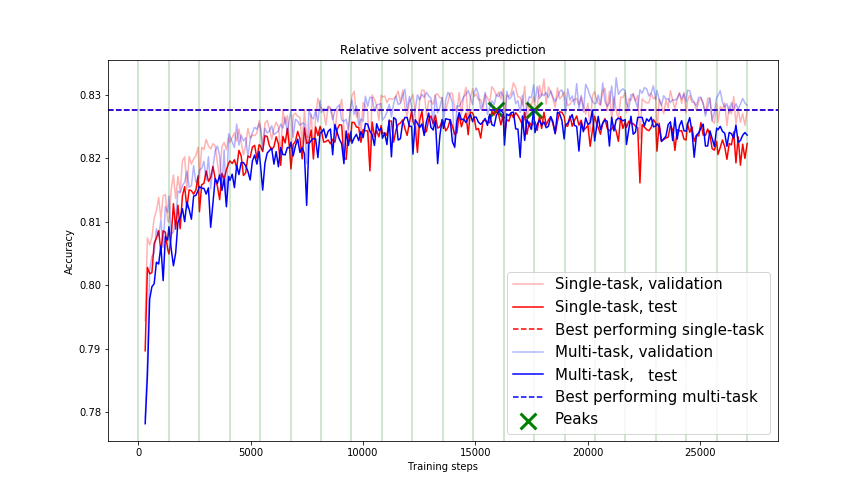
\includegraphics[width=\linewidth]{../graphs/final/rel_final_small}
  \caption{Peak performance on the relative solvent accessibility. Green lines represent epochs.}
\end{figure}

\begin{table}[h]
\centering
\begin{tabular}{lclcl}
 & \multicolumn{4}{c}{\textbf{Absolute Solvent Accessibility}} \\
 & \multicolumn{2}{c}{\textit{Validation}} & \multicolumn{2}{c|}{\textit{Test}} \\ \cline{2-5} 
 & \multicolumn{1}{l}{Epoch} & \multicolumn{1}{l|}{Accuracy} & \multicolumn{1}{l}{Epoch} & Accuracy \\
Single-task & 12 & \multicolumn{1}{l|}{81.671\%} & 11 & 81.006\% \\
Multi-task & 11 & \multicolumn{1}{l|}{81.636\%} & 10 & 80.912\%
\end{tabular}
\end{table}

\begin{figure}[H]
  \centering
  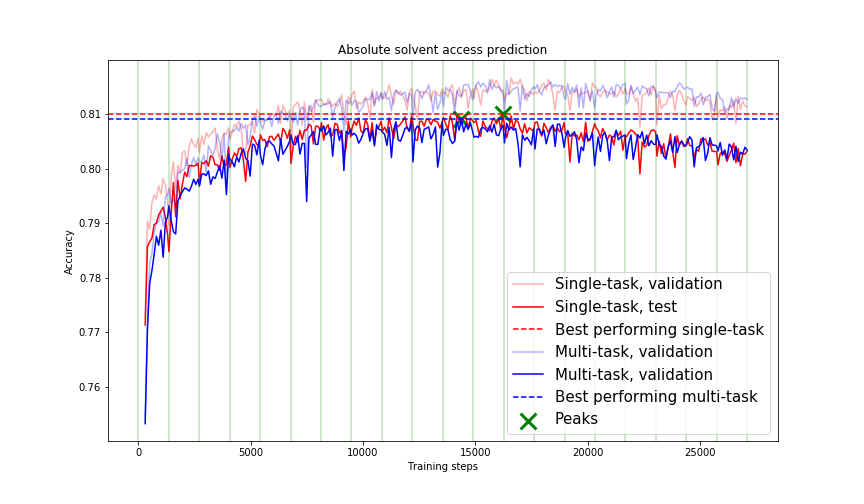
\includegraphics[width=\linewidth]{../graphs/final/abs_final_small}
  \caption{Peak performance on the absolute solvent accessibility.}
\end{figure}

\noindent It becomes clear that the the decisions made about the parameters throughout our process were indeed made on the basis of optimizing the accuracy on the validation set. Further, the results here seem to indicate that there are noteworthy differences between the test and validation sets.\\
As is also the case for predicting the secondary structures, the effects of overfitting are seen quite clearly. In most of the runs the models reach their predictive ceiling already around 12 or 13 epochs, before losing accuracy on the test and validations sets again as the model starts overfitting to the training set.
%\begin{table}[]
%\centering
%\begin{tabular}{lclll}
%\multicolumn{1}{c}{\textbf{}} & \multicolumn{4}{c}{\textbf{Solvent Accessibility}} \\
% & \multicolumn{2}{c}{{\ul Single-task}} & \multicolumn{2}{c}{{\ul Multi-task}} \\
% & Epoch & \multicolumn{1}{c}{Accuracy} & \multicolumn{1}{c}{Epoch} & \multicolumn{1}{c}{Accuracy} \\ \cline{2-5} 
%\multicolumn{1}{l|}{Feature} & \multicolumn{4}{c|}{\textit{Validation set}} \\
%\multicolumn{1}{l|}{Relative} & \multicolumn{1}{l}{13} & \multicolumn{1}{l|}{83.245\%} & 15 & \multicolumn{1}{l|}%{83.263\%} \\
%\multicolumn{1}{l|}{Absolute} & \multicolumn{1}{l}{12} & \multicolumn{1}{l|}{81.671\%} & 11 & \multicolumn{1}{l|}%{81.636\%} \\ \cline{2-5} 
%\multicolumn{1}{l|}{} & \multicolumn{4}{c|}{\textit{Test set}} \\
%\multicolumn{1}{l|}{Relative} & \multicolumn{1}{l}{11} & \multicolumn{1}{l|}{82.752\%} & 12 & \multicolumn{1}{l|}%{82.763\%} \\
%\multicolumn{1}{l|}{Absolute} & \multicolumn{1}{l}{11} & \multicolumn{1}{l|}{81.006\%} & 10 & \multicolumn{1}{l|}%{80.912\%}
%\end{tabular}
%\end{table}

\subsubsection{Secondary Structures}
By implementing multi-task learning in the model we saw a slight increase in the accuracy when predicting protein secondary structures as compared to the single-task model. We did however observe that while the two models both moved towards predictive ceilings not that far apart, the multi-task model reached it significantly faster.
\begin{table}[h]
\centering
\begin{tabular}{lclcl}
 & \multicolumn{4}{c}{\textbf{Secondary Structures Q8}} \\
 & \multicolumn{2}{c|}{\textit{Validation}} & \multicolumn{2}{c}{\textit{Test}} \\ \cline{2-5} 
 & \multicolumn{1}{l}{Epoch} & \multicolumn{1}{l|}{Accuracy} & \multicolumn{1}{l}{Epoch} & Accuracy \\
Single-task & 17 & \multicolumn{1}{l|}{71.410\%} & 19 & 71.239\% \\
Multi-task & 12 & \multicolumn{1}{l|}{71.558\%} & 11 & 71.566\%
\end{tabular}
\end{table}

\begin{figure}[H]
  \centering
  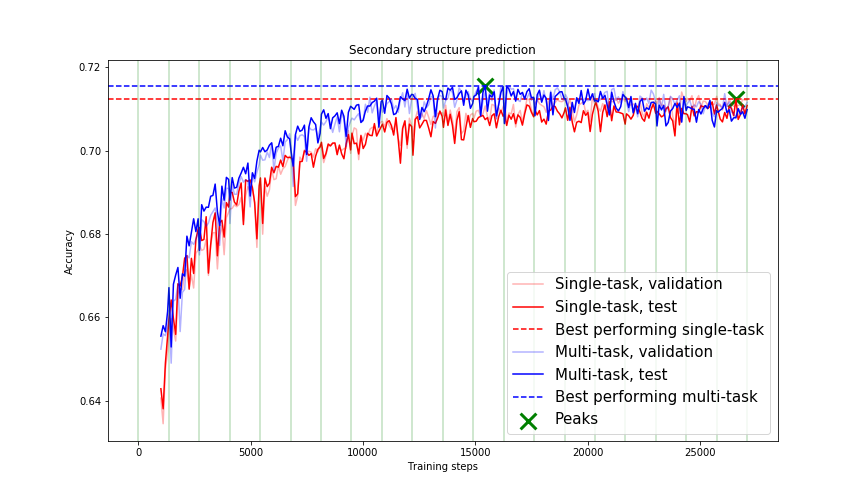
\includegraphics[width=\linewidth]{../graphs/final/final_secondary_small}
  \caption{Peak performance on the absolute solvent accessibility.}
\end{figure}

\newpage
\begin{multicols}{2}






















\section{Conclusion}
The aim this paper was to put to test the question of whether applying multi-task learning to a convolutional neural network could help improve its accuracy in regards to predicting protein secondary structures.\\
To do this we built first a single-task model predicting Q8 secondary structures from amino acid recidues as well as the sequence profiling, as well as a similar model for predicting relative and absolute solvent accessibility.\\
We then built another model combining these two elements in a hard parameter-sharing multi-task learning neural network, and optimized this with regards to hyperparameters number of layers, learning rate, layer depth and kernel size.\\
Training these three models with the optimized parameters showed that while the single-task model was slightly better at predicting solvent accessibilities, the multi-task model did indeed outperform the single-task when it came to predicting secondary structures.\\
At the offset of this project we used articles by \textbf{CITER ALLE ARTIKLERNE}, noting that authors Wang et al. had also built a convolutional neural network (DeepCNF-SS) with the same goals, reaching a Q8 accuracy of 75.2\% on the same data set as we have used, while we with our model only achieved 71.24\% on our single-task and 71.57\% on our multi-task models. Differences between DeepCNF-SS and our single-task model include both use use of regularization and the use of a Conditional Random Field as a precursive layer. \\
Since our results showed an increase in accuracy when expanding the scope of the model to multi-task learning, one can speculate if a similar increase in performance could be expected if one was to implement multi-task learning into Wang et al.'s superior model.

Modellen blev ikke bedre, men blev nogenlunde god til både at forudsige struktur og solvent-egenskaber.
Vi kan have nogle overvejelser omkring hvad vi kunne have gjort bedre, f.eks:
\begin{itemize}
\item Gaussisk filtrering over dataen
\item Evt. soft parameter sharing
\item Regularization hvis vi tør
\item En anden opbygning af multi-modellen hvor der var et enkelt eller flere fully-connected layers til solvent-egenskaberne.
\end{itemize}


\section{Appendix}

\section*{Amino acids}
\begin{table}[h]
\caption{Amino acids}
\centering
\begin{tabular}{l|l}
Letter	& Amino Acid	\\ \hline
A		& Alanine		\\
C		& Cysteine		\\
D		& Aspartic Acid	\\
E		& Glutamic Acid	\\
F		& Phenylalanine	\\
G		& Glycine		\\
H		& Histidine		\\
I		& Isoleucine	\\
K		& Lysine		\\
L		& Leucine		\\
M		& Methionine	\\
N		& Asparagine	\\
P		& Proline		\\
Q		& Glutamine		\\
R		& Arginine		\\
S		& Serine		\\
T		& Threonine		\\
V		& Valine		\\
W		& Tryptophan	\\
Y		& Tyrosine		\\

\end{tabular}
\end{table}

\newpage
\section*{Batch sizes}
A comparison of achieved accuracies on the validation and test set respectively performed on the unoptimized multi-task model can be seen below.
\begin{table}[H]
\centering
\begin{tabular}{lllllll}
\multicolumn{7}{c}{Layer depth = 80, kernel size = 11, learning rate = 0.00025, 3 hidden layers}                                                                                                                                                                                                                                                                                   \\ \hline
           & \multicolumn{3}{c|}{Validation set}                                                                                                                                                               & \multicolumn{3}{c}{Test set}                                                                                                                                      \\ \hline
Batch size & Q8 & \begin{tabular}[c]{@{}l@{}}Relative\\solvent\\accessibility\end{tabular} & \multicolumn{1}{l|}{\begin{tabular}[c]{@{}l@{}}Absolute\\solvent\\accessibility\end{tabular}} & Q8 & \begin{tabular}[c]{@{}l@{}}Relative\\ solvent\\ accessibility\end{tabular} & \begin{tabular}[c]{@{}l@{}}Absolute\\ solvent\\accessibility\end{tabular} \\ \hline
1          & 71.25\%     & 82.98\%                                                                       & \multicolumn{1}{l|}{81.41\%}                                                                       & 70.973\%    & 82.184\%                                                                   & 80.572\%                                                                \\
2          & 71.25\%     & 82.76\%                                                                       & \multicolumn{1}{l|}{81.21\%}                                                                       & 70.951\%    & 82.523\%                                                                   & 80.847\%                                                                \\
4          & 70.25\%     & 82.28\%                                                                       & \multicolumn{1}{l|}{80.84\%}                                                                       & 70.438\%    & 82.103\%                                                                   & 80.570\%                                                                \\
8          & 69.42\%     & 82.51\%                                                                       & \multicolumn{1}{l|}{80.73\%}                                                                       & 69.557\%    & 82.012\%                                                                   & 80.319\%                                                                \\
16         & 68.15\%     & 82.15\%                                                                       & \multicolumn{1}{l|}{80.42\%}                                                                       & 68.459\%    & 81.595\%                                                                   & 79.924\%                                                                \\
32         & 66.94\%     & 81.61\%                                                                       & \multicolumn{1}{l|}{79.85\%}                                                                       & 67.279\%    & 81.196\%                                                                   & 79.483\%                                                                \\
64         & 65.10\%     & 80.97\%                                                                       & \multicolumn{1}{l|}{79.25\%}                                                                       & 65.100\%    & 80.644\%                                                                   & 78.899\%                                                               
\end{tabular}
\end{table}

\section*{Layer depth}

\begin{figure}[H]
  \centering
  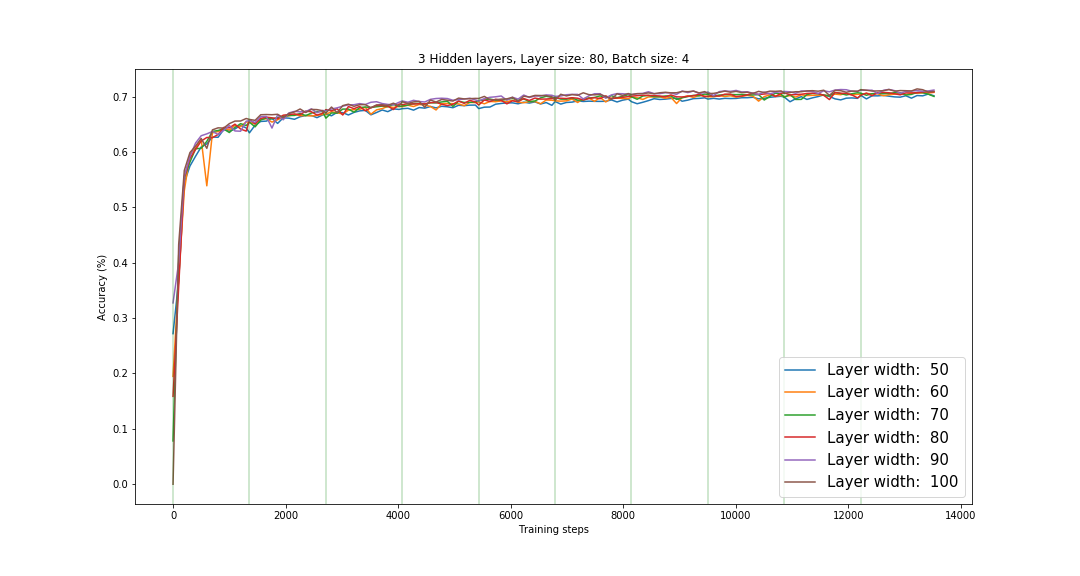
\includegraphics[width=\linewidth]{../graphs/new/layer_width_2}
  \caption{Accuracy on the validation set with varying layer depth.}
\end{figure}

\section*{Kernel sizes}

\begin{figure}[H]
  \centering
  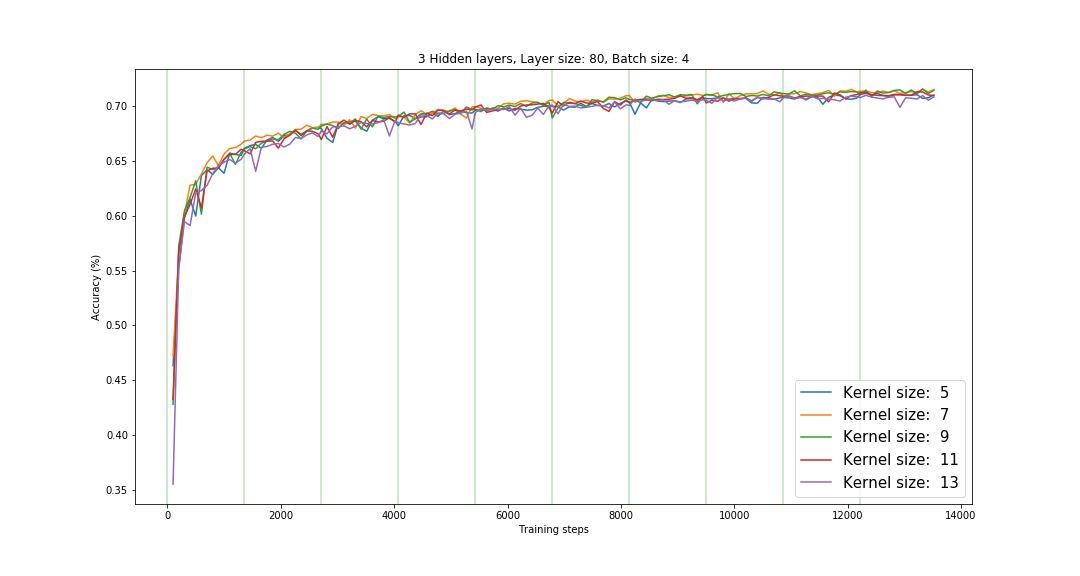
\includegraphics[width=\linewidth]{../graphs/new/kernel_size_1}
  \caption{All of the tested values for constant kernel size.}
\end{figure}

\bibliography{sample} 
\bibliographystyle{apalike}
\end{multicols}
\end{document}